% -*- TeX -*- -*- UK -*-
% ----------------------------------------------------------------
\documentclass[10pt]{article}
%\usepackage[printfigures]{figcaps}
%\usepackage[nolists,nomarkers]{endfloat}
%Preamble:
\usepackage{a4wide}
\input{sl_preamble.tex}
\hypersetup{colorlinks,linkcolor=blue,citecolor=teal,urlcolor=teal}
\input{sl_graphics_preamble.tex}
\graphicspath{{"Figures/"}}
%
\usepackage{array}
%\newcounter{tablerow}[table]
%\newcommand{\tablerowautorefname}{row}
%\newenvironment{tabularn}[1]{\begin{tabular}{#1>{\refstepcounter{tablerow}}l}}{\end{tabular}}
%\usepackage{etoolbox}
%\AtBeginEnvironment{tabular}{\setcounter{tablerow}{0}}
\renewcommand{\figurename}{Appendix-figure}
\renewcommand{\figureautorefname}{Appendix-figure}
\DeclareCaptionLabelFormat{supp}{\textbf{#1 #2}}
\captionsetup{labelformat=supp}
% ----------------------------------------------------------------
% New commands etc.
\input{sl_definitions.tex}
\input{sl_symbols.tex}
%matrices
\newcommand{\I}{\mathbf{I}}
%vec of ones
%equilibrium distribution
\newcommand{\pr}{\mathbf{p}}
\newcommand{\eq}{\pr^\infty}
%other symbols
\newcommand{\w}{\mathbf{w}}
\newcommand{\W}{\mathbf{W}}
\newcommand{\frg}{\W^\mathrm{F}}
\newcommand{\M}{\mathbf{M}}
\newcommand{\F}{\boldsymbol{\Phi}}
\newcommand{\pot}{^{\text{pot}}}
\newcommand{\dep}{^{\text{dep}}}
\newcommand{\potdep}{^{\text{pot/dep}}}
\newcommand{\norm}{_0}
\newcommand{\inc}{_{\text{inc}}}
\newcommand{\dec}{_{\text{dec}}}
\newcommand{\incdec}{_{\text{inc/dec}}}
\newcommand{\wt}{_{\text{WT}}}
\newcommand{\ko}{_{\text{K$^\mathrm{b}$D$^\mathrm{b}$-/-}}}
\newcommand{\KO}{K$^\mathrm{b}$D$^{\mathrm{b}-/-}$}
%\newcommand{\ko}{_{\text{MHC}}}
%\newcommand{\KO}{MHC}
\newcommand{\tpre}{t_{\text{pre}}}
\newcommand{\ttrain}{t_{\text{train}}}
%\newcommand{\lmax}{_{\text{max}}}
%\newcommand{\lmin}{_{\text{min}}}
\newcommand{\modelfig}[1][A]{Figure 3#1 of the main text}
\newcommand{\datafig}[1][B]{Figure 2#1 of the main text}
\newcommand{\chrfig}[1][B]{Figure 4#1 of the main text}
\newcommand{\compfig}[1][A]{Figure 4 -- figure supplement 2#1}
\newcommand{\basefig}{Figure 1 -- figure supplement 2}
% ----------------------------------------------------------------
%
%%%%%%%%%%%%%%%%%%%%%%%%%%%%%%%%%%%%%%%%%%%%%%%%%%%%%%%%%%%%%%%%%%%%%%%%%%
% Title info:
\title{Appendix to ``Understanding both enhanced and impaired learning with enhanced plasticity: a saturation hypothesis''}
%
%% Author List:
%%
%\author{An Author$^a$, Another Author$^b$ and Yet Another Author$^c$\\
%%
%\small{\emph{$^a$ Address 1}}\\
%\small{\emph{$^b$ Address 2}}\\
%\small{\emph{$^c$ Address 3}}\\
%}
\author{}
\date{}

\begin{document}

%\setcounter{page}{8}
%\setcounter{figure}{7}
\maketitle


%%%%%%%%%%%%%%%%%%%%%%%%%%%%%%%%%%%%%%%%%%%%%%%%%%%%%%%%%%%%%%%%%%%%%%%%%%


%\begin{abstract}
%  We see if we can model VOR gain increase and decrease learning in mice with a knockout in MHC as well as wild-type.
%\end{abstract}

%\tableofcontents
%\listoffigures

%%%%%%%%%%%%%%%%%%%%%%%%%%%%%%%%%%%%%%%%%%%%%%%%%%%%%%%%%%%%%%%%%%%%%%%%%%
% Beginning of Article:
%%%%%%%%%%%%%%%%%%%%%%%%%%%%%%%%%%%%%%%%%%%%%%%%%%%%%%%%%%%%%%%%%%%%%%%%%%

\section{Mathematical formalism}\label{sec:setup}


\subsection{Models of synapses}\label{sec:synapse}

We make the following assumptions:
\begin{itemize}
  \item There synapses are identical and have $M$ internal functional states, where the states of different synapses are independent of each other.
%  \item The synapses that are eligible for plasticity are chosen randomly.
  \item Candidate potentiating/depressing plasticity event timings are distributed as Poisson processes with rates $r\potdep$.
  \item Candidate potentiation and depression events are described by Markov processes with transition probabilities $\M\potdep$.
  \item The synaptic weights of the internal states are given by the column vector $\w$. This can only take values in a finite range that we can shift to $\pm1$. Most of the models will only use the two extreme values.
\end{itemize}

The overall rate of candidate plasticity events will only affect the units we measure time in.
For the questions we are investigating, qualitative understanding of when learning is enhanced/impaired rather than detailed numerical matching of learning curves, this is completely irrelevant.
Only the relative rates will matter.
With this in mind, we define
%
\begin{equation}\label{eq:fpotdep}
  r = r\pot + r\dep,
  \qquad
  f\pot = \frac{r\pot}{r},
  \qquad
  f\dep = \frac{r\dep}{r},
\end{equation}
%
where $f\potdep$ is the fraction of candidate plasticity events that are potentiating/depressing.

The independence and identicalness of synapses means that the state of the system can be completely described by the probability distribution over the internal states, the \emph{row} vector $\pr(t)$ which evolves as
%
\begin{equation}\label{eq:evolve}
  \diff{\pr(t)}{t} = r\pr(t)\frg,
  \qquad
  \frg = f\pot\M\pot+f\dep\M\dep-\I,
\end{equation}
%
where $\frg$ is a continuous time Markov transition matrix and $\I$ is the identity matrix.
Eventually, this will settle into the equilibrium distribution:
%
\begin{equation}\label{eq:eqprob}
  \eq\frg = \mathbf{0}.
\end{equation}
%

%For models with only two possible synaptic weights, the distribution of synaptic weights is completely described by the mean, $\pr(t)\w$.

We model the \KO\ mice by changing $\M\dep\wt$ to $\M\dep\ko$, which has larger off-diagonal matrix elements.
This makes it easier to induce a decrease in synaptic weight, modelling the observed lower threshold for LTD \cite{McConnell2009MHCcerebellum}.

We will look at several different models,
the serial model (see \cite{Leibold2008serial,Ben-DayanRubin2007sparse} and \autoref{fig:models}\ref{fig:serial_model}) which has only two values for the synaptic weight,
the two-state model (which can be thought of as a special case of the serial model, see \autoref{fig:models}\ref{fig:binary_model}),
the multistate model (see \cite{amit1994learning,Fusi2007multistate} and \autoref{fig:models}\ref{fig:multistate_model}) which has a linearly varying synaptic weight,
and the cascade model (see \cite{Fusi2005cascade} and \autoref{fig:models}\ref{fig:cascade_model}).
We will also look at a new, pooled resource model that we will define below in \autoref{sec:pooledmodel} and a non-uniform version of the multistate model that we will describe in \autoref{sec:nonunimodel}.

For the serial, multistate and two state models, we will use the same value for the transition probabilities, $q$, for potentiation in the wild-type and \KO\ models.
We will use a larger value for $q$ for depression in the \KO\ models than in the wild-type.

For the cascade model, we will use the same value for the parameter $x$ (which controls the decay of transition rates, see \cite{Fusi2005cascade}) for potentiation in the wild-type and \KO\ models.
We will use a larger value for $x$ for depression in the \KO\ models than in the wild-type.

The values used for all these parameters in simulations are listed in \autoref{fig:sim_results}\ref{tab:params}.

\begin{figure}
 \begin{center}
   \begin{myenuma}
  \begin{tabular}{l@{\hspace{0.05\linewidth}}l}
    \item\aligntop{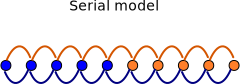
\includegraphics[height=1.7cm]{serial.svg}}\label{fig:serial_model}&
    \item\aligntop{\includegraphics[height=1.7cm]{binary.svg}}\label{fig:binary_model}\\[1.7cm]
    \item\aligntop{\includegraphics[height=1.7cm]{multistate.svg}}\label{fig:multistate_model}&
    \item\aligntop{\includegraphics[height=2.5cm]{cascade.svg}}\label{fig:cascade_model}\\[2.5cm]
    \item\aligntop{\includegraphics[height=2.3cm]{pooled.svg}}\label{fig:pooled_model}&
    \item\aligntop{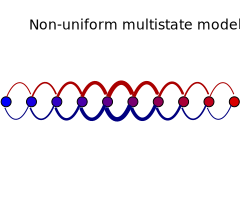
\includegraphics[height=2.3cm]{multistate_nonuni.svg}}\label{fig:nonuni_model}
  \end{tabular}
   \end{myenuma}
 \end{center}
  \caption[Transition probabilities for different models]{{Transition probabilities for different models.}
  Potentiation induces transitions indicated by orange arrows, depression indicated by blue arrows.
  States of strong/weak synaptic weight indicated by orange/blue circles.
  (\ref{fig:serial_model}) In the serial model the transition probabilities for potentiation/depression are all equal and it is parameterised by these two values.
  The synaptic weight takes only two values, $\pm1$.
  (\ref{fig:binary_model}) The two-state model is parameterised by the two transition probabilities.
  (\ref{fig:multistate_model}) In the multistate model the transition probabilities for potentiation/depression are all equal and it is parameterised  by these two values.
  The synaptic weight varies linearly in the interval $[-1,1]$.
  (\ref{fig:cascade_model}) In the cascade model, the transition probabilities decay geometrically with a parameter $x$ (see \cite{Fusi2005cascade}) and synaptic weight takes only two values.
  (\ref{fig:pooled_model}) In the pooled resource model,
  Several two-state synapses share resources that are required for potentiation and depression.
  These resources are depleted as more synapses are potentiated or depressed.
  This pool of synapses can be modelled as one compound synapse.
  (\ref{fig:nonuni_model}) In the non-uniform multistate model
  the synaptic weight varies linearly in the interval $[-1,1]$, similar to the multistate model, but the transition probabilities between adjacent states decays exponentially away from the central transition for both potentiation and depression.
  } \label{fig:models}
\end{figure}

\subsubsection{Pooled resource model}\label{sec:pooledmodel}

Suppose that there is some resource required for potentiation/depression that is shared between $P$ synapses and is depleted as more synapses are potentiated/depressed and replenished when this is reversed, as shown in \autoref{fig:models}\ref{fig:pooled_model}.
We can avoid going beyond the independent synapse model by modelling this pool of synapse as a single compound synapse.

We will model the individual synapses with the two-state model.
Let $i=0\ldots P$ be the number of them that are potentiated.
We will model the effect of resource depletion linearly with the potentiation/depression probabilities for the individual synapses:
%
\begin{equation}\label{eq:depletion}
  \begin{aligned}
    q\pot &= \frac{(P-i-1)q\lmax + i\,q\lmin}{P-1}, \quad& i &= 0 \ldots P-1,\\
    q\dep &= \frac{(i-1)q\lmax + (P-i)q\lmin}{P-1}, & i &= 1 \ldots P.
  \end{aligned}
\end{equation}
%
At each plasticity event for the compound synapse, one of the individual synapses will be chosen randomly for update.
This effectively reduces the transition probabilities by $1/P$.

This compound synapse would seem to have $2^P$ internal states.
However, we need only keep track of the number of potentiated synapses, not their identity, leaving $M=P+1$ states.
The transition network will then have a multistate topology (see \autoref{fig:models}\ref{fig:multistate_model}) but the transition probabilities will no longer be uniform and the weight of the compound synapse is the mean of its constituent synapses:
%
\begin{equation}\label{eq:pooledweight}
  \w_i = \frac{2i}{P}-1.
\end{equation}
%


The Markov process is lumpable \wrt this partition of states (see \cite{kemeny1960finite,burke1958markovian,Ball1993Lumpability}).
The transition probabilities between lumps $i$ and $j$ is computed by choosing one state from lump $i$ and summing the transition probabilities to all states in lump $j$,
which must be the same for all states in lump $i$.

For any state in lump $i$, there are $P-i$ synapses that can be potentiated to go to lump $i+1$.
Each of these transition probabilities is $q\pot/P$.
Similarly, there are $i$ synapses that can be depressed to go to lump $i-1$.
Each of these transition probabilities is $q\dep/P$.
Thus:
%
\begin{equation}\label{eq:pooledpotdep}
  \begin{aligned}
    \M\pot_{ii+1} &=  \brk{\frac{(P-i-1)q\lmax + i\,q\lmin}{P-1}} \frac{P-i}{P} ,
      \quad& i &= 0 \ldots P-1,\\
    \M\dep_{ii-1} &=  \brk{\frac{(i-1)q\lmax + (P-i)q\lmin}{P-1}} \frac{i}{P} ,
           & i &= 1 \ldots P,
  \end{aligned}
\end{equation}
%
with all other off-diagonal elements equal to zero.
The diagonal elements are chosen so that the rows sum to one.

This model is parameterised by the range of values, $q\in[q\lmin,q\lmax]$, for potentiation and depression.
We will use the same values for potentiation in the wild-type asnd \KO\ models.
We will use larger values for depression in the \KO\ models than in the wild-type.
we consider a version of this model that has resource depletion for depression only, so that potentiation transition probabilities are unaffected by the number of potentiated synapses.
This is done by setting $q\pot\lmax=q\pot\lmin$.
The values of these parameters are listed in \autoref{fig:sim_results}\ref{tab:params}.


%\begin{figure}
% \begin{center}
%  \aligntop{\includegraphics[height=4cm]{pooled.svg}}
% \end{center}
%  \caption[The pooled resource model]{The pooled resource model.
%  Several two-state synapses share resources that are required for potentiation and depression.
%  These resources are depleted as more synapses are potentiated or depressed.
%  This pool of synapses can be modelled as one compound synapse.} \label{fig:pooled_model}
%\end{figure}


\subsubsection{Non-uniform multistate model}\label{sec:nonunimodel}

This model, shown in \autoref{fig:models}\ref{fig:nonuni_model}, is similar to the multistate model (see \autoref{fig:models}\ref{fig:multistate_model})), as it only has transitions between adjacent states and a linearly varying synaptic weight.
However, like the cascade model (see \cite{Fusi2005cascade} and \autoref{fig:models}\ref{fig:cascade_model}), the transition probabilities decay exponentially away from the central transition.
More precisely:
%
\begin{equation}\label{eq:nonunidef}
    \M\pot_{ii+1} = \M\dep_{i+1i} =  x^{\abs{\frac{M+1}{2}-i}+\half},
      \quad i = 1 \ldots M-1,
\end{equation}
%
with all other off-diagonal elements equal to zero.
The diagonal elements are chosen so that the rows sum to one.

This model is parameterised by the values of $x$ chosen for potentiation and depression.
We will use a larger value for depression in the \KO\ models.
The values used are listed in \autoref{fig:sim_results}\ref{tab:params}.



%\begin{figure}
% \begin{center}
%  \aligntop{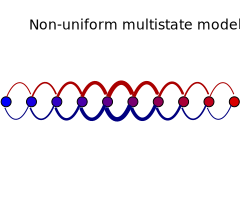
\includegraphics[height=3cm]{multistate_nonuni.svg}}
% \end{center}
%  \caption[The non-uniform multistate model]{The non-uniform multistate model.
%  Similar to the multistate model, (\autoref{fig:models}\ref{fig:multistate_model}), the synaptic weight varies linearly in the interval $[-1,1]$, but the transition probabilities between adjacent states decays exponentially away from the central transition for both potentiation and depression.} \label{fig:nonuni_model}
%\end{figure}


%%%%%%%%%%%%%%%%%%%%%%%%%%%%%%%%%%%%%%%%%%%%%%%%%%%%%%%%%%%%%%%%%%%%%%%%%%



\subsection{Model of VOR learning experiment}\label{sec:learning}

Training the animal will not change the internal dynamics of a synapse under potentiation or depression.
It will change the environment, which will lead to a change in how often potentiation and depression occur.
%It could be manifested in a change in which synapses are potentiated/depressed, but this could not be captured in this type of model.
We will model this by changing $f\potdep$, leaving $\M\potdep$ unchanged.
This approach was used to model motor learning in \cite{Smith2006savings}.

The untrained case will be described by $f\dep=f\dep\norm$.
Gain-increase training  will be described by $f\dep=f\dep\inc>f\dep\norm$, and
gain-decrease training  will be described by $f\dep=f\dep\dec<f\dep\norm$.
Note that the forgetting matrix \eqref{eq:evolve} and the equilibrium distribution \eqref{eq:eqprob} depend on $f\dep$, which we will indicate with subscripts.

Before training, the synaptic distribution will be in the equilibrium distribution corresponding to $f\dep\norm$.
During gain-increase training, it will evolve according to \eqref{eq:evolve} with $f\pot\inc$:
%
\begin{equation}\label{eq:nopre}
  \pr(t) = \eq\norm \exp\prn{rt\frg\inc}.
\end{equation}
%
On the other hand, if the gain-increase training follows gain-decrease pre-training for some time period, $\tpre$:
%
\begin{equation}\label{eq:withpre}
  \pr(t) = \eq\norm \exp\prn{r\tpre\frg\dec} \exp\prn{r(t-\tpre)\frg\inc}.
\end{equation}
%

We will describe the effect of training by the decrease in mean synaptic weight:
%
\begin{equation}\label{eq:learning}
  L(t) = \prn{\pr(0)-\pr(t)}\w.
\end{equation}
%
One can approximate the input to a Purkinje cell as some linear combination of the synaptic weights (weighted by the activities of the corresponding parallel fibres).
If we are not keeping track of synaptic identity, the most natural linear combination to use would be an equal sum of them all.
The behavioural output (VOR gain) will be some unknown, non-linear function of the synaptic weights, so the best we can hope for is to reproduce qualitative features of the experiment, such as whether learning is enhanced or impaired by the mutation or pre-training.

As the knockout produces no change in baseline performance, there must be a compensatory mechanism somewhere else.
We will model this compensation as a simple linear offset, as could be produced by another population of neurons/synapses whose effect cancels with these neurons/synapses.

We will assume $f\dep\wt=f\dep\ko$.
This is because the relevant effects of the knockout are well localised to the Purkinje cells, as shown by the rescue data, so the activity of the parallel and climbing fibres should not change very much.
Therefore the rates of potentiation and depression should not change very much either.
%This implies that the mean synaptic weight in equilibrium differs between the \KO\ models and wild type, but that is also suggested by the data regarding basal levels of phospho-GluR2 at serine 880.

For the most part, we set $f\dep\norm=\half$, $f\dep\inc=f\dep\norm+\Delta f$ and $f\dep\dec=f\dep\norm-\Delta f$, with $\Delta f>0$.
We use the same values for wild-type and \KO\ models for the reasons discussed above.
%We will mostly treat gain-increase and decrease symmetrically, but this is not necessary.
We could adjust $r$ to keep $r\pot$ unchanged, if so desired, but this would only change the overall timescale and would not affect any of the qualitative comparisons that we are concerned with here.
The values of these parameters are listed in \autoref{fig:sim_results}\ref{tab:params}.

We are also assuming that the relation between VOR gain and mean synaptic weight is the same for \KO\ mice and wild-type, except for a linear offset to compensate for the difference in equilibrium weights mentioned above.
This ensures that the qualitative questions mentioned above (enhancement or impairment of learning) will not be affected.


%%%%%%%%%%%%%%%%%%%%%%%%%%%%%%%%%%%%%%%%%%%%%%%%%%%%%%%%%%%%%%%%%%%%%%%%%%




\section{Simulation and analysis of models}\label{sec:results}

The features of the experiments shown in \modelfig\ that we'd like to capture are:
%
\begin{enumerate}
  \item Without pre-training, gain-increase learning is significantly faster in the wild-type than in the \KO\ mice.
  \item For the wild-type, gain-increase learning is significantly faster without pre-training than with it.
  \item For the \KO\ mice, gain-increase learning is significantly faster with pre-training than without it.
  \item After pre-training, gain-increase learning is significantly faster in the \KO\ mice than in the wild-type.
%  \item Gain-decrease pre-training is slightly faster in the wild-type, but not significantly so.\label{it:gaindown}
\end{enumerate}
%
These questions will not be affected by any output nonlinearity, as long as it is monotonic and fixed.
\emph{We will not study gain-decrease learning}, as its mechanisms are not fully understood, and known to be different to to gain-increase.
We are only modelling the effect of gain-decrease training on \emph{these} synapses.
We will also not discuss the curvature of the learning curves, as this can be changed by the nonlinear relation between synaptic weight and VOR gain.
%However, both the wild-type and \KO\ mice should be affected in the same way, so the difference in the curvature of the \KO\ mice and wild-type curves after pre-training would be nice to capture.

We will try to gain some analytic insight to some of these models by looking at the slope of the learning curve at the start of gain-increase training.
This is proportional to the net-flux from the states with strong synaptic weight to the weaker states, measured using the transition rates for gain-increase but the equilibrium distribution for either untrained or gain-decrease, assuming that pre-training lasts long enough to reach the equilibrium distribution for gain-decrease.
%This should be multiplied by the difference in synaptic weights.
%But, as this quantity is constant within a model and doesn't change when comparing wild-type and \KO\ models or with/without pre-training, it can be ignored.

The learning curves resulting from these simulations can be found in \autoref{fig:sim_results}.
The values for all parameters we will use can be found in \autoref{fig:sim_results}\ref{tab:params}.

\begin{figure}[p]
\begin{myenuma}
  \begin{tabular}{lll}
      \item\label{fig:serial_sim}
      \aligntop{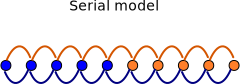
\includegraphics[width=0.24\linewidth]{serial.svg}}
      &
      \item\label{fig:binary_sim}
      \hspace{0.05\linewidth}\aligntop{\includegraphics[width=0.12\linewidth]{binary.svg}}
      &
      \item\label{fig:multistate_sim}
      \aligntop{\includegraphics[width=0.24\linewidth]{multistate.svg}}
      \\[1.3cm]
      \aligntop{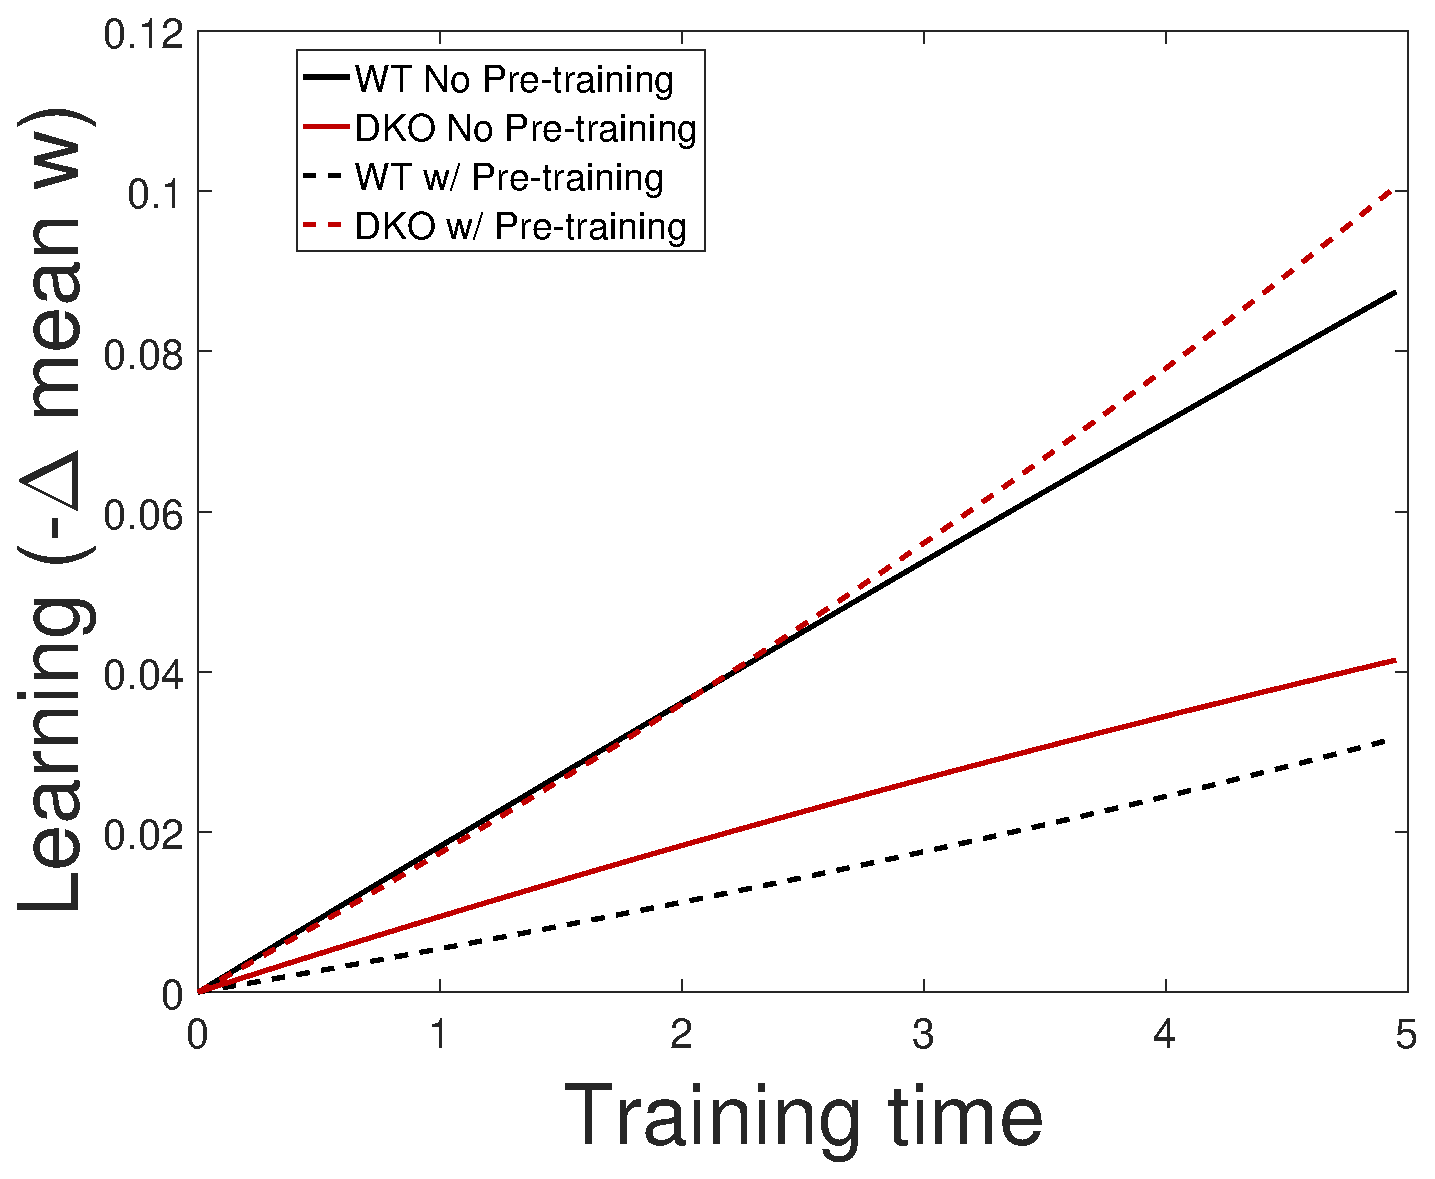
\includegraphics[width=0.29\linewidth]{serial_fit_learnS.eps}}
      &
      \aligntop{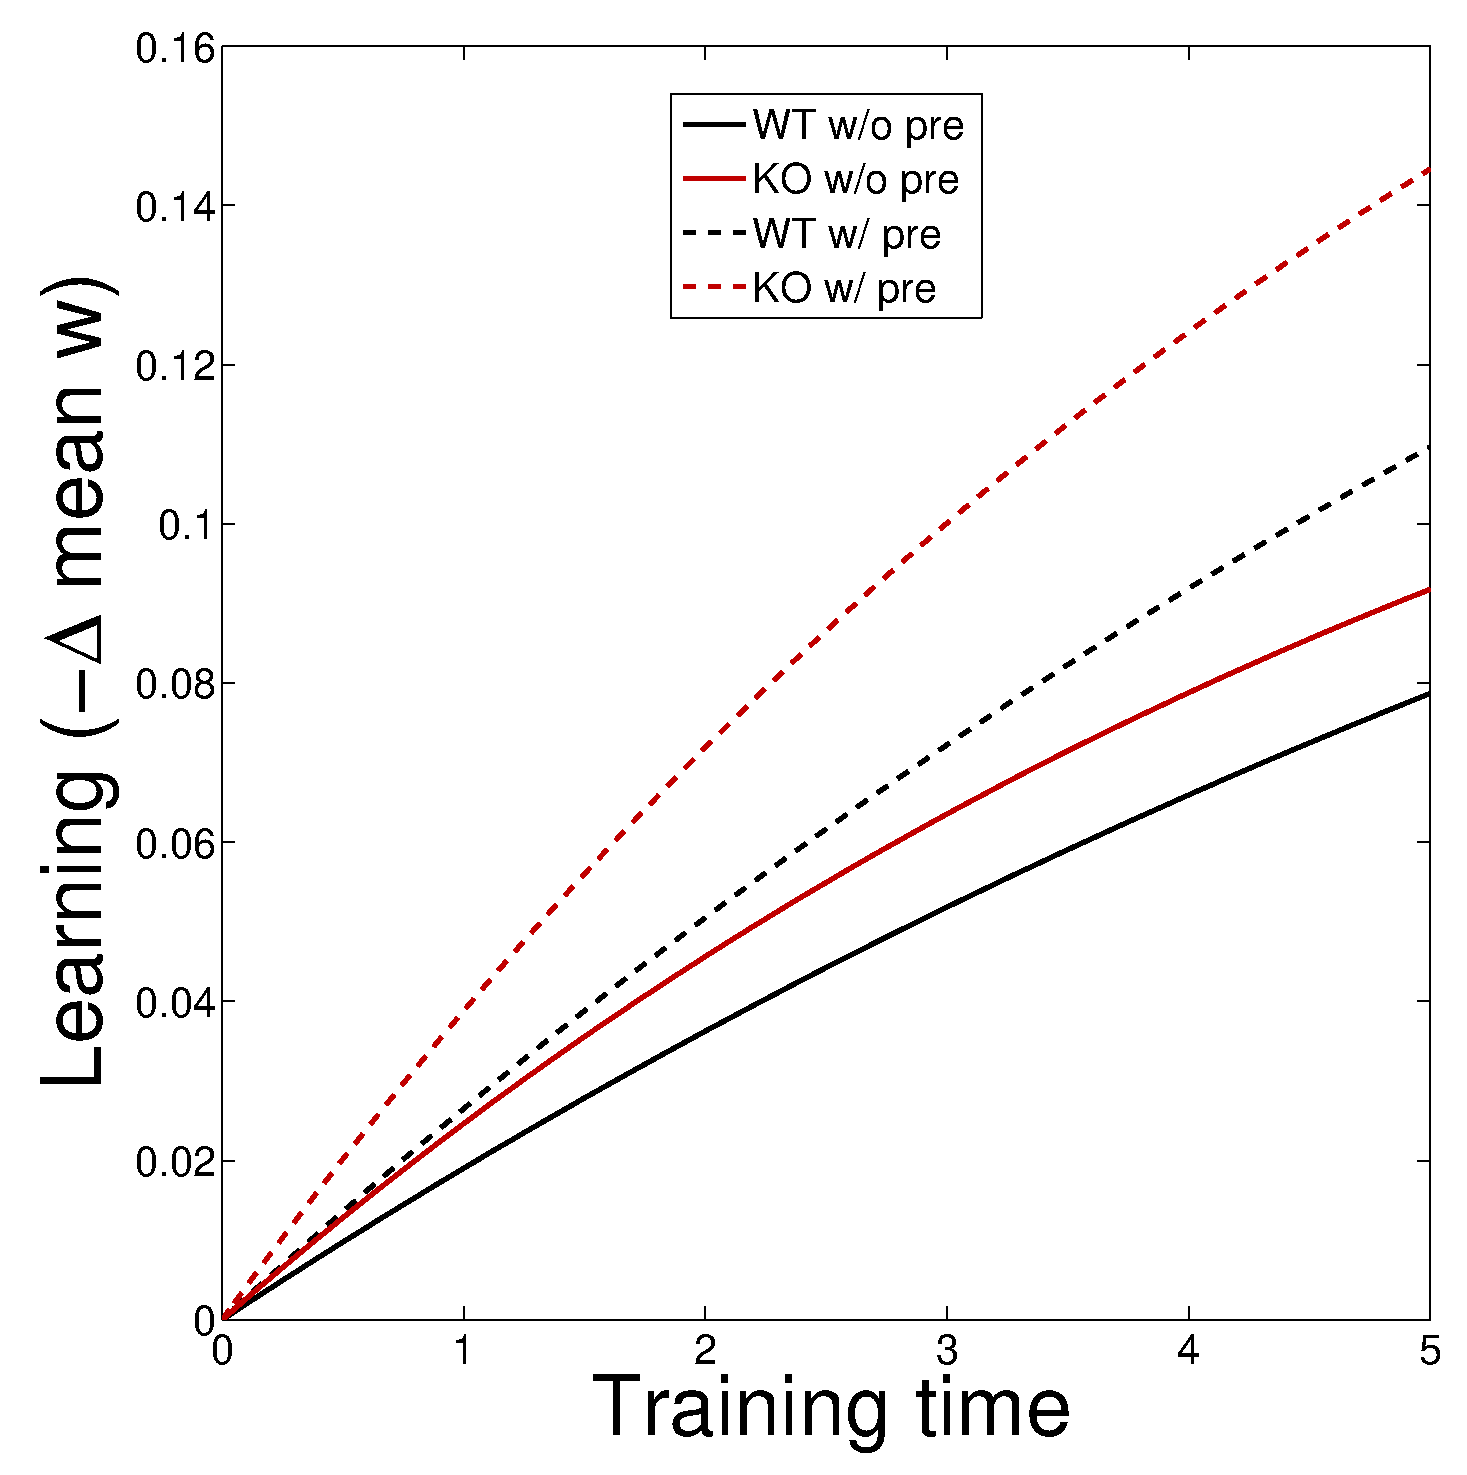
\includegraphics[width=0.29\linewidth]{binary_learnS.eps}}
      &
      \aligntop{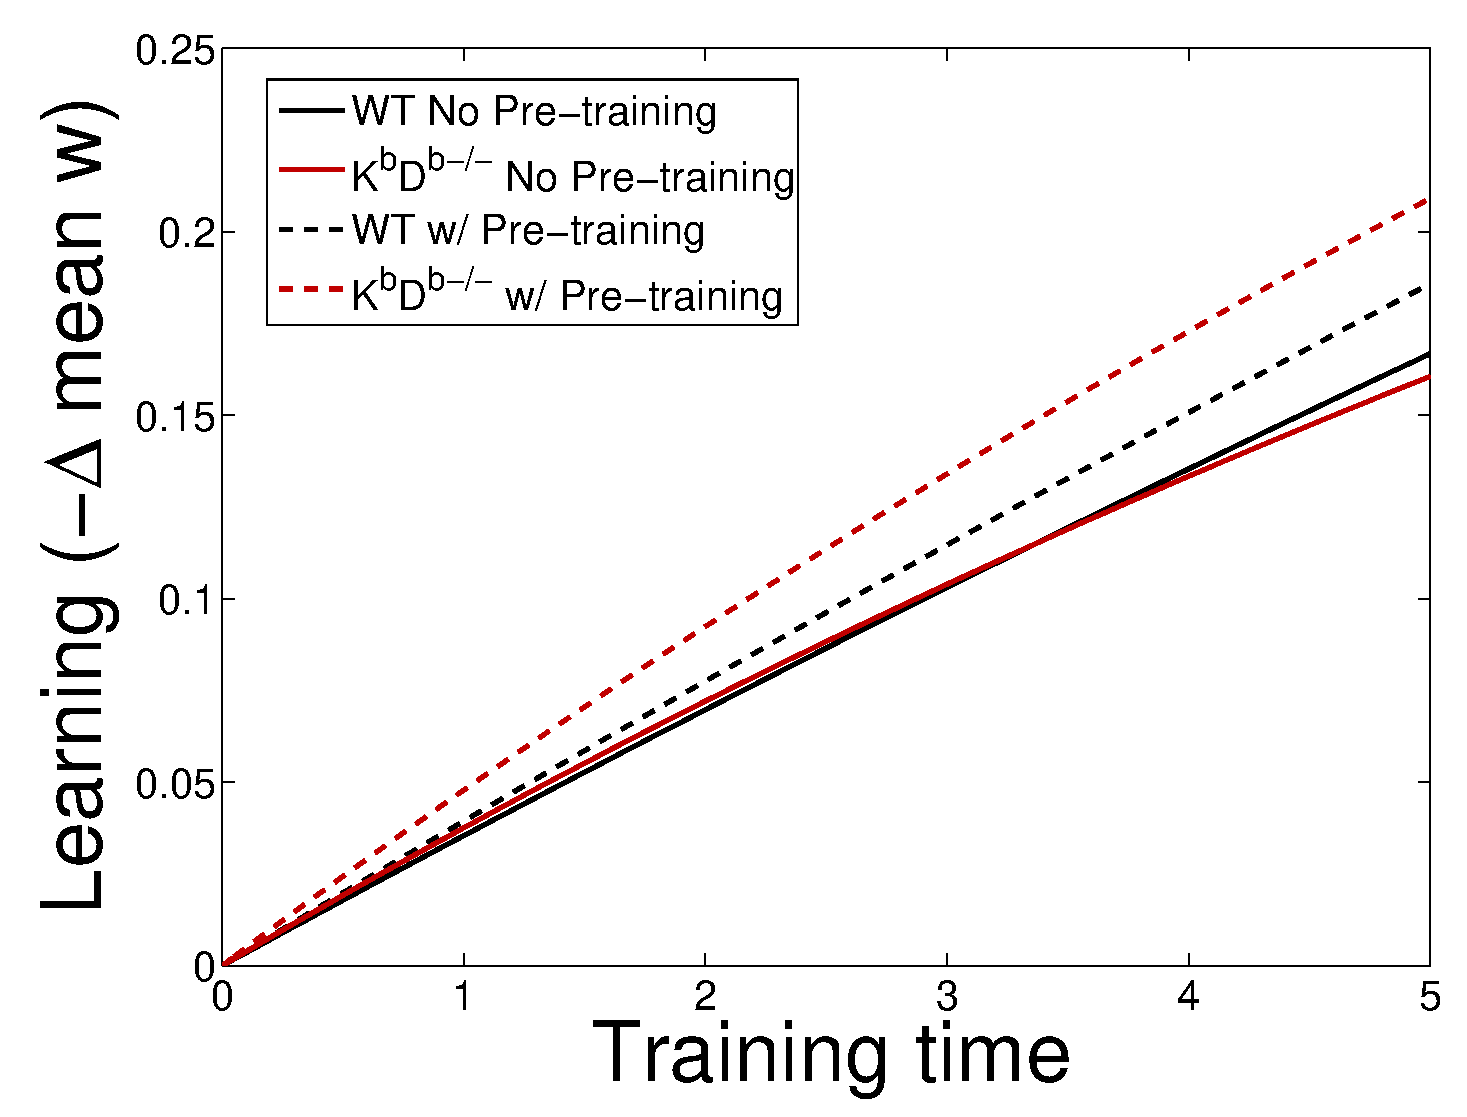
\includegraphics[width=0.29\linewidth]{multistate_lin_learnS.eps}}
      \\[3.5cm]
      \item\label{fig:pooled_sim}
      \aligntop{\includegraphics[width=0.29\linewidth]{pooled_deponly.svg}}
      &
      \item\label{fig:cascade_sim}
      \aligntop{\includegraphics[width=0.24\linewidth]{cascade.svg}}
      &
      \item\label{fig:nonuni_sim}
      \aligntop{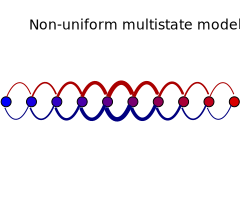
\includegraphics[width=0.24\linewidth]{multistate_nonuni.svg}}
      \\[1.8cm]
      \aligntop{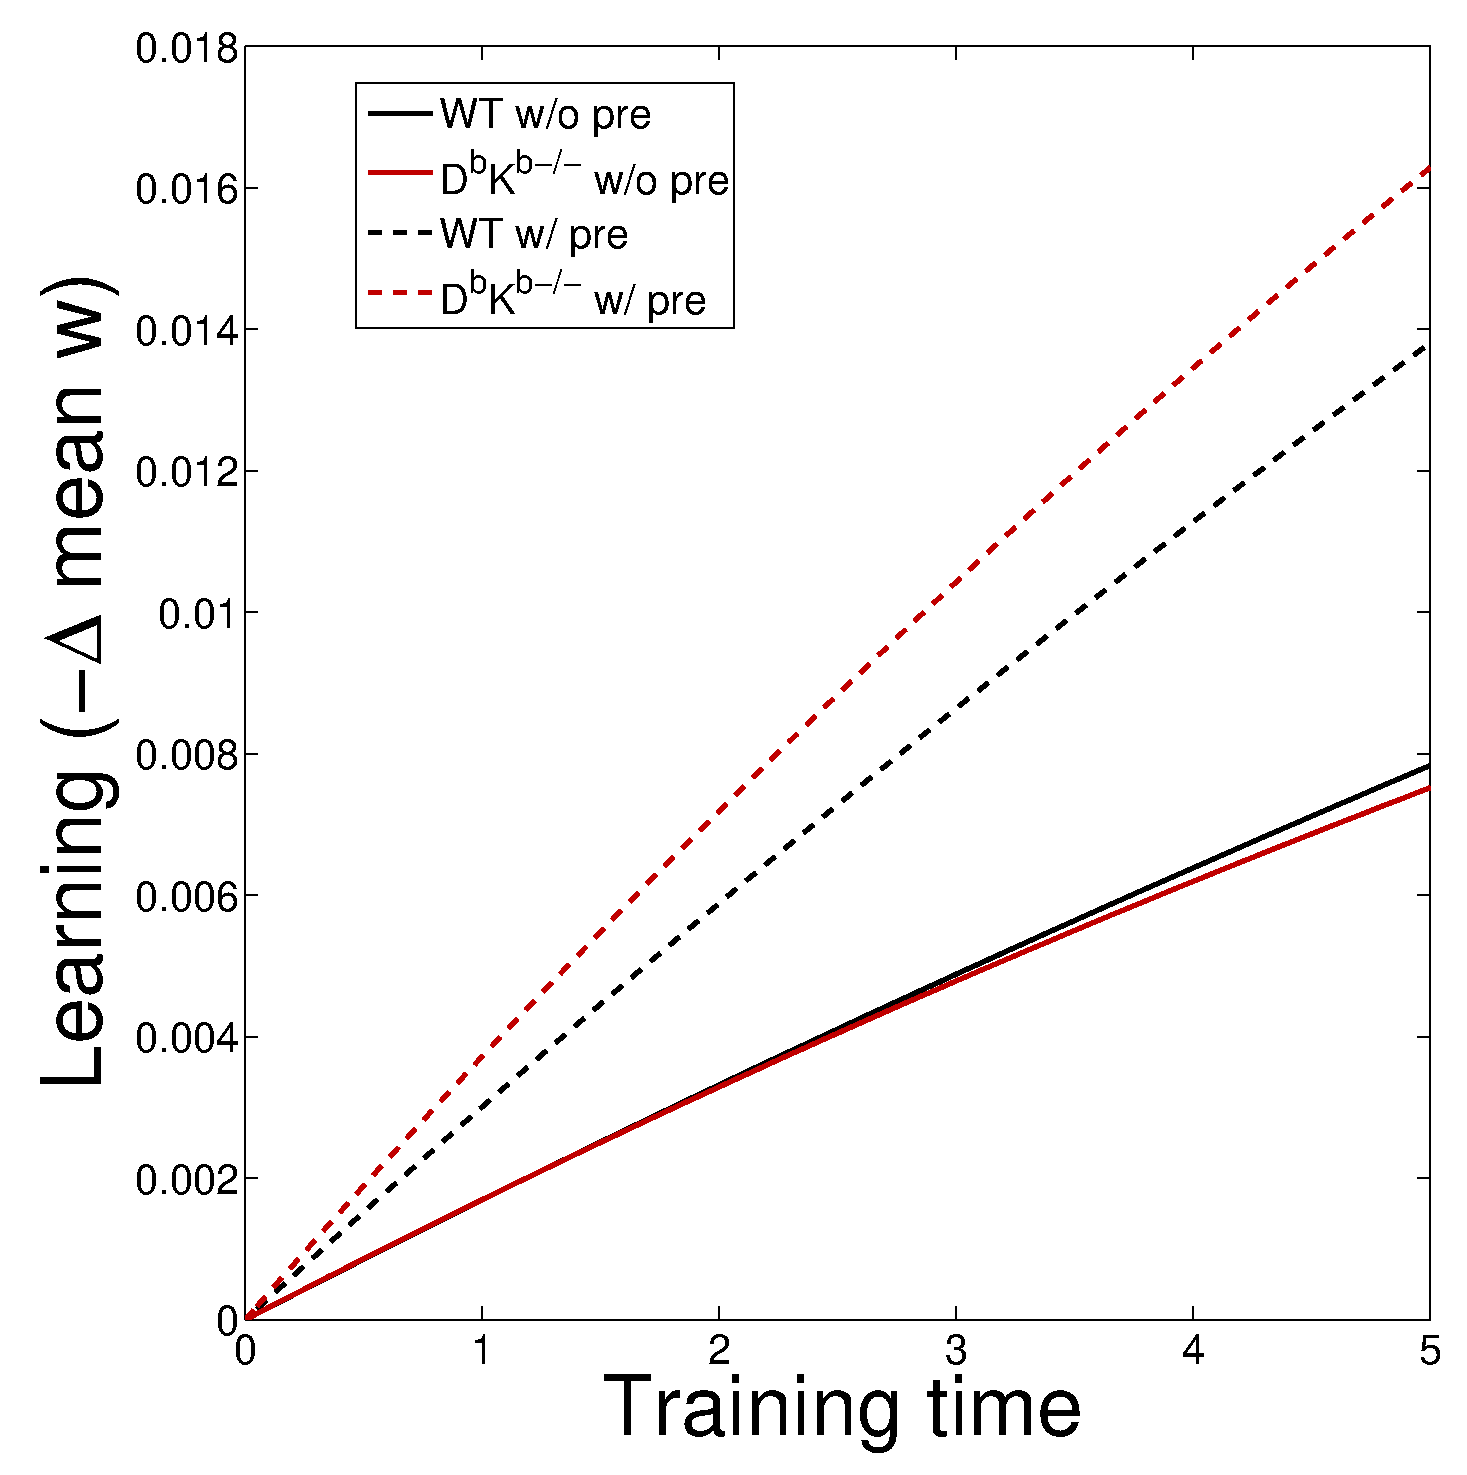
\includegraphics[width=0.29\linewidth]{pooled_deponly_learnS.eps}}
      &
      \aligntop{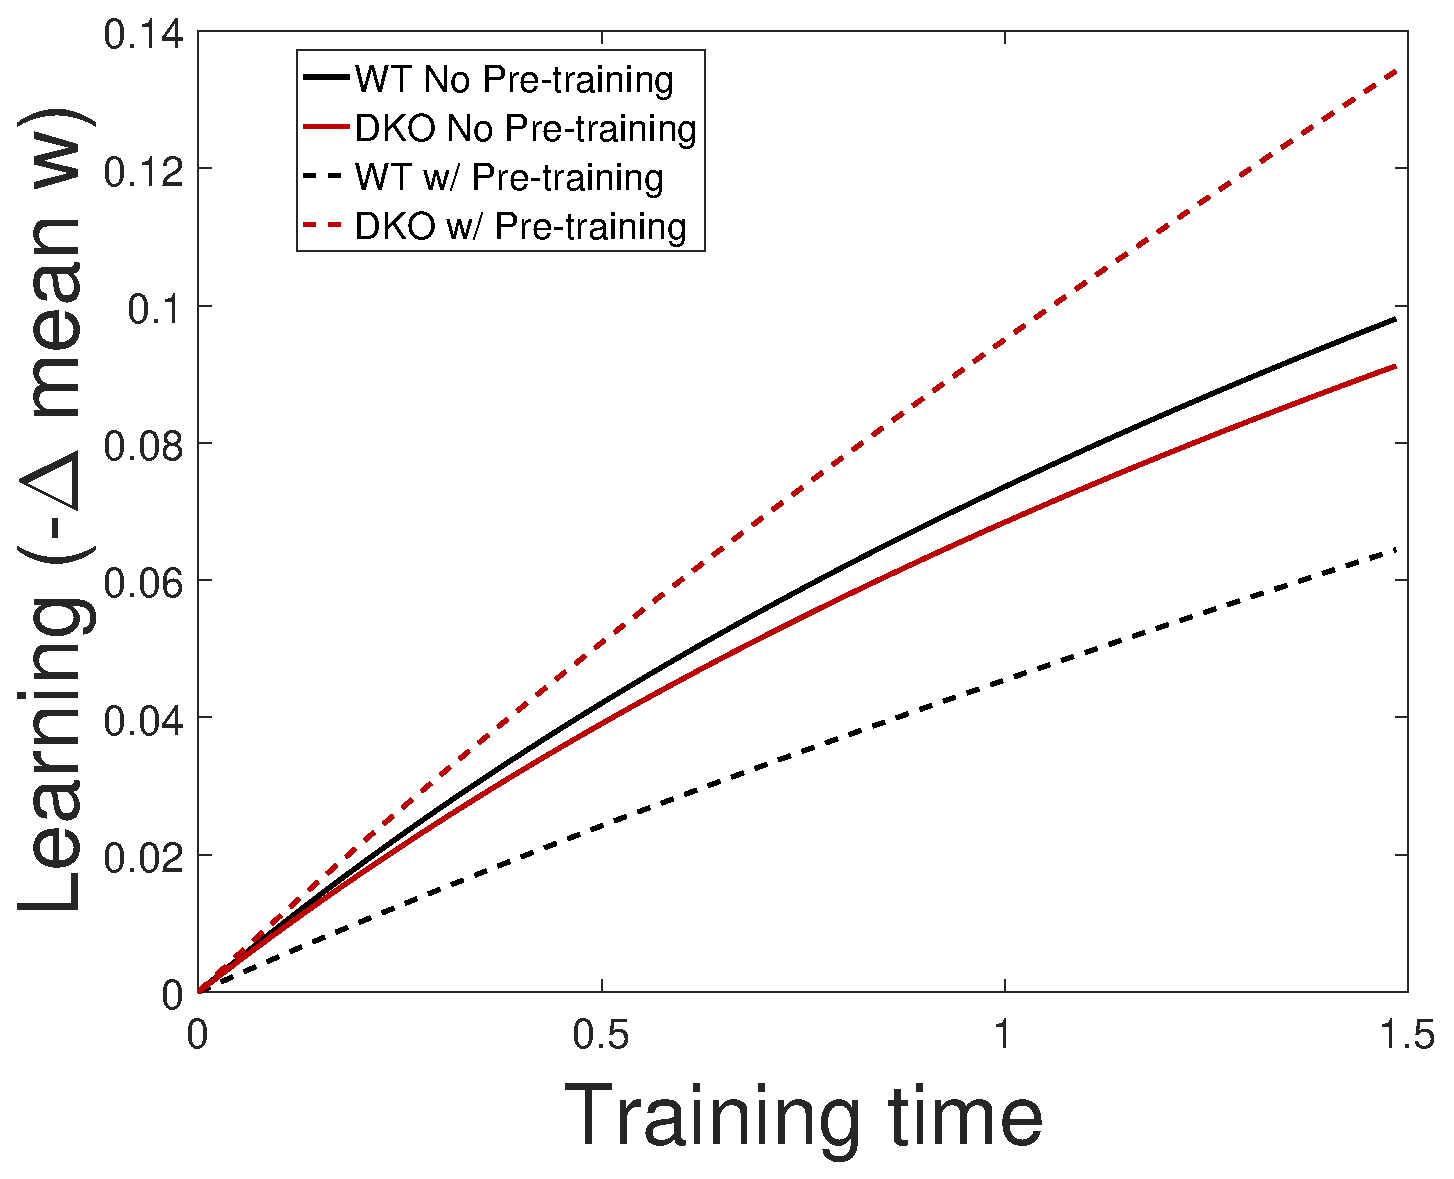
\includegraphics[width=0.29\linewidth]{cascade_fit_learnS.eps}}
      &
      \aligntop{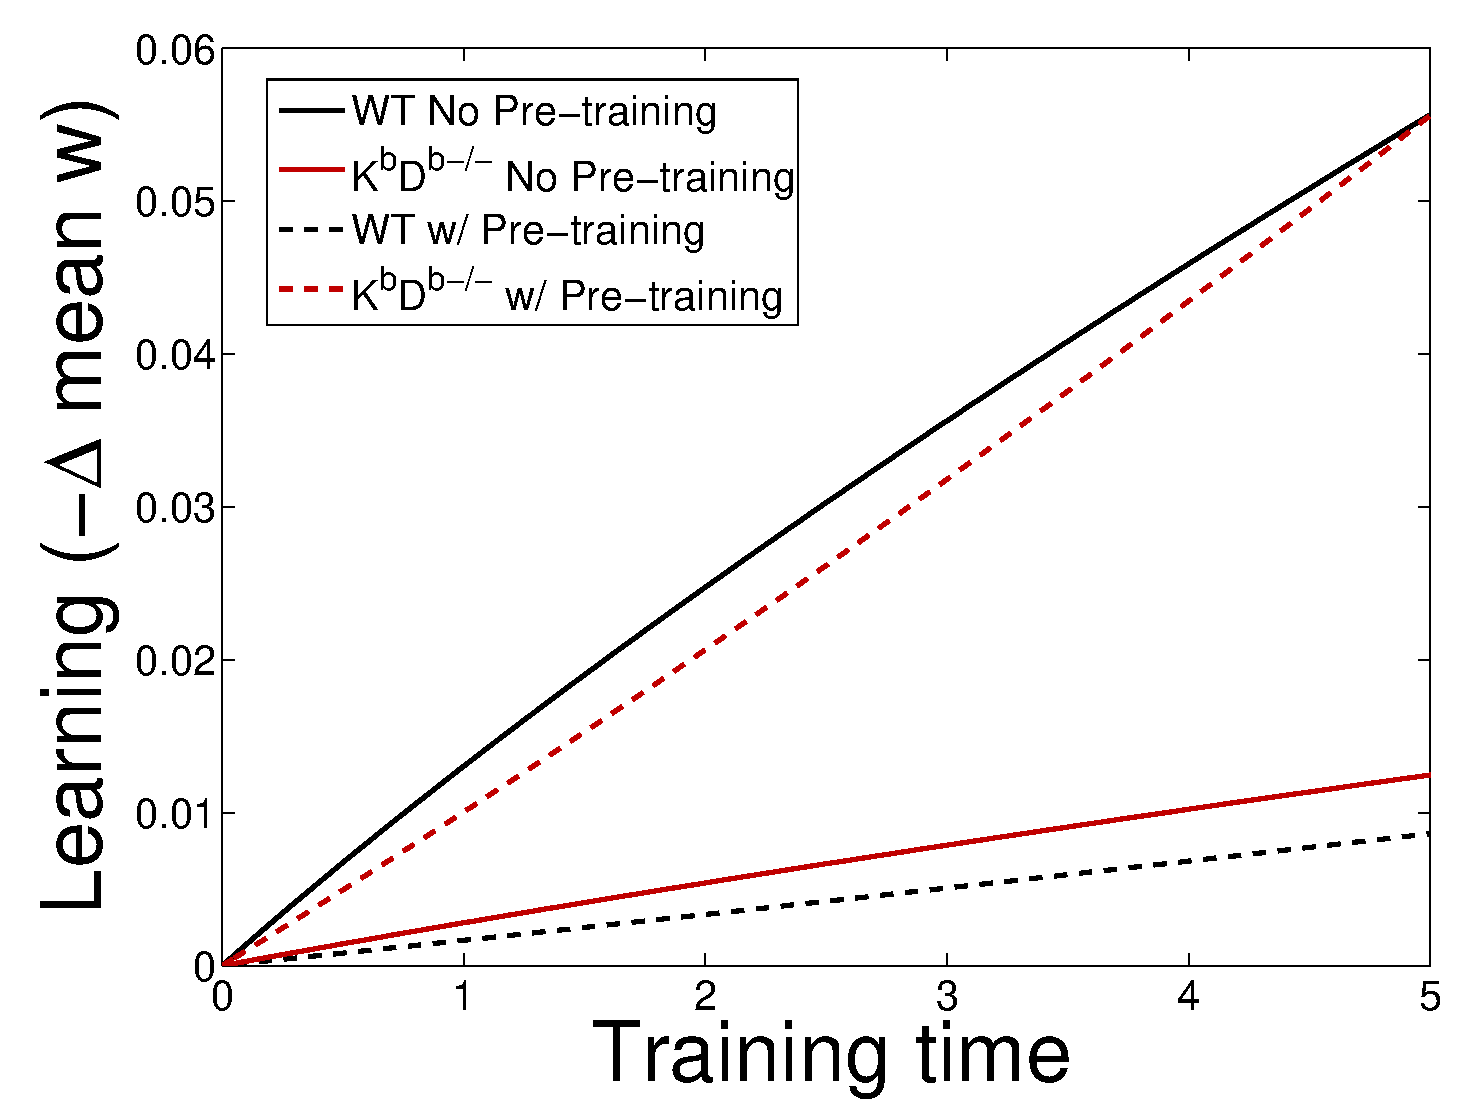
\includegraphics[width=0.29\linewidth]{nonuni_fit_learnS.eps}}
  \end{tabular}

  \vspace{0.5cm}
  \item\label{tab:params}\aligntop{
  \begin{tabular}{|l|c|c|c|c|c|c|c|c|}
    \cline{1-9}
    % after \\: \hline or \cline{col1-col2} \cline{col3-col4} ...
    Model & \#  & \multicolumn{3}{c|}{Plasticity parameter} & \multicolumn{3}{c|}{$f\dep$} & $r\tpre$ \\
    \cline{3-8}
    & states & pot & WT dep & {\footnotesize\KO} dep & base & inc & dec & {} \\

    \cline{1-9}
    Serial   & 10 & $0.12$  & $0.14$  & $0.2$  & 0.5 & 0.89 & 0.11  & 100  \\%&\label{tr:serial_fit} \\
    Two-state     & 2  & $0.1$  & $0.1$  & $0.2$  & 0.5 & 0.6 & 0.4  & 5   \\%&\label{tr:binary} \\
    Multistate    & 10 & $0.3$  & $0.3$  & $0.4$  & 0.5 & 0.8 & 0.2  & 5   \\%&\label{tr:multistate_lin} \\
    Pooled res.\ & 7  & $0.008$        & $[0.0006,0.6]$  & $[0.001,1]$
                                          & 0.5 & 0.9 & 0.1 & 20 \\%&\label{tr:pooled_deponly}\\
    Cascade  & 14 & $0.386$  & $0.398$  & $0.466$  & 0.522 & 0.63 & 0.002  & 200  \\%&\label{tr:cascade_fit} \\
    Non-uni.\ & 12 & $0.4$    & $0.4$    & $0.53$   & 0.5 & 0.7 & 0.1 & 500  \\%&\label{tr:nonuni_fit} \\
    \cline{1-9}
  \end{tabular}}
  \end{myenuma}
  \caption[Simulation results for various models]{(\ref{fig:serial_sim}-\ref{fig:nonuni_sim}) Simulation results for various models, showing decrease in mean synaptic weight over time during gain increase training from the normal state (solid) and after gain-decrease pre-training (dashed) for wild-type (black) and \KO\ (red) models.
  (\ref{tab:params}) Parameters used for simulations.
  For the serial, two state and multistate models, the plasticity parameter listed is the transition probability between adjacent states.
  For the pooled resource model, the plasticity parameters are the minimum and maximum transition probability for the constituent two-state synapses.
  For the cascade and non-uniform multistate models, the plasticity parameter is the ratio of adjacent transition probabilities.}\label{fig:sim_results}
\end{figure}


%\begin{table}
% \begin{center}
%  \begin{tabularn}{|l|c|c|c|c|c|c|}
%    \cline{1-7}
%    % after \\: \hline or \cline{col1-col2} \cline{col3-col4} ...
%    Model & \# states & pot & WT dep & \KO\ dep & $\Delta f$ & $r\tpre$ \\
%    \cline{1-7}
%%    Serial        & 10 & $q=0.3$  & $q=0.3$  & $q=0.4$  & 0.1  & 20  &\label{tr:multistate_weak} \\
%    Serial        & 10 & $q=0.3$  & $q=0.3$  & $q=0.4$  & 0.3  & 20  &\label{tr:multistate_med} \\
%%    Serial        & 10 & $q=0.3$  & $q=0.3$  & $q=0.4$  & 0.45 & 30  &\label{tr:multistate_strong} \\
%    Two-state     & 2  & $q=0.1$  & $q=0.1$  & $q=0.2$  & 0.1  & 5   &\label{tr:binary} \\
%    Multistate    & 10 & $q=0.3$  & $q=0.3$  & $q=0.4$  & 0.3  & 5   &\label{tr:multistate_lin} \\
%%    Pooled        & 10 & $q\in[0.3,0.4]$  & $q\in[0.3,0.4]$  & $q\in[0.6,0.8]$
%%                                          & 0.1 & 20 &\label{tr:pooled_plenty}\\
%%    Pooled        & 10 & $q\in[0.05,0.4]$ & $q\in[0.05,0.4]$  & $q\in[0.1,0.8]$
%%                                          & 0.1 & 20 &\label{tr:pooled_scarce}\\
%    Pooled res. & 7  & $q=0.008$        & $q\in[0.0006,0.6]$  & $q\in[0.001,1]$
%                                          & 0.4 & 20 &\label{tr:pooled_deponly}\\
%%    Cascade       & 10 & $x=0.25$ & $x=0.25$ & $x=0.33$ & 0.3  & 20  &\label{tr:cascade_short} \\
%    Cascade       & 10 & $x=0.25$ & $x=0.25$ & $x=0.33$ & 0.3  & 100 &\label{tr:cascade_long} \\
%    Non-uni. MS& 10 & $x=0.25$ & $x=0.25$ & $x=0.33$ & 0.3  & 150 &\label{tr:nonuni} \\
%    \cline{1-7}
%%   \hline
%%    % after \\: \hline or \cline{col1-col2} \cline{col3-col4} ...
%%    & Model & \# states & pot,WT dep & \KO\ dep & $\Delta f$ & $r\ttrain$ & $r\tpre$ \\
%%    \cline{1-7}
%%    \label{tr:cascade_short}&
%%    Cascade    & 10 & $x=0.25$ & $x=0.33$ & -0.3 & 50 & 50   \\
%%    \label{tr:cascade_long}&
%%    Cascade    & 10 & $x=0.25$ & $x=0.33$ & -0.3 & 50 & 150  \\
%%    \label{tr:multistate_weak}&
%%    Multistate & 10 & $q=0.6$  & $q=0.8$  & -0.1 & 50 & 50   \\
%%    \label{tr:multistate_strong}&
%%    Multistate & 10 & $q=0.6$  & $q=0.8$  & -0.4 & 20 & 20   \\
%%    \label{tr:binary}&
%%    Two-state  & 2  & $q=0.4$  & $q=0.8$  & -0.1 & 5  & 5    \\
%%    \label{tr:pooled_plenty}&
%%    Pooled     & 10 & $q\in[0.3,0.4]$  & $q\in[0.6,0.8]$
%%                                          & -0.1 & 70 & 70 \\
%%    \label{tr:pooled_scarce}&
%%    Pooled     & 10 & $q\in[0.1,0.4]$  & $q\in[0.2,0.8]$
%%                                          & -0.1 & 70 & 70 \\
%%    \cline{1-7}
%  \end{tabularn}
% \end{center}
%  \caption{Parameters used for simulations in \autoref{fig:sim_results}.} \label{tab:params}
%\end{table}

%\newcommand{\arrangefig}[1]{\begin{center}
% \begin{myenuma}
%  \item\aligntop{\includegraphics[width=7cm]{#1_learn.eps}}\label{fig:#1_learn}
%  \item\aligntop{\includegraphics[width=7cm]{#1_learnS.eps}}\label{fig:#1_learnS}
%  \\ \vp\vp
%  \item\label{fig:#1_eq}\begin{myenumi}
%                    \item\aligntop{\includegraphics[width=7cm]{#1_eq_WT.eps}}\label{fig:#1_eq_WT}
%                    \item\aligntop{\includegraphics[width=7cm]{#1_eq_KO.eps}}\label{fig:#1_eq_KO}
%                  \end{myenumi}
%  \\ \vp \vp
%  \item\label{fig:#1_pr}\begin{myenumi}
%                    \item\aligntop{\includegraphics[width=3cm]{#1_pr_WT_nopre.eps}}\label{fig:#1_pr_WT_nopre}
%                    \item\aligntop{\includegraphics[width=3cm]{#1_pr_WT_pre.eps}}\label{fig:#1_pr_WT_pre}
%                    \item\aligntop{\includegraphics[width=3cm]{#1_pr_KO_nopre.eps}}\label{fig:#1_pr_KO_nopre}
%                    \item\aligntop{\includegraphics[width=3cm]{#1_pr_KO_pre.eps}}\label{fig:#1_pr_KO_pre}
%                  \end{myenumi}
% \end{myenuma}
% \end{center}}
%
%\newcommand{\captiontext}[1]{ can be found in \autoref{tr:#1} of \autoref{tab:params}.
%  Time is measured in units of $1/r$, the mean time between plasticity events.
%  (\ref{fig:#1_learn}) Learning curves for wild-type and \KO\ models with and without pre-training.
%  (\ref{fig:#1_learnS}) Learning curves restricted to gain-increase training.
%  (\ref{fig:#1_eq}) Equilibrium distributions without training or with gain-increase/decrease training for (\ref{fig:#1_eq_WT}) wild-type and (\ref{fig:#1_eq_KO}) \KO\ models,
%  with states of weak synaptic strength to the left and strong states to the right.
%  (\ref{fig:#1_pr}) Evolution of probability distributions for (\ref{fig:#1_pr_WT_nopre},\ref{fig:#1_pr_WT_pre}) wild-type and  (\ref{fig:#1_pr_KO_nopre},\ref{fig:#1_pr_KO_pre}) \KO\ models without (\ref{fig:#1_pr_WT_nopre},\ref{fig:#1_pr_KO_nopre}) and with (\ref{fig:#1_pr_WT_pre},\ref{fig:#1_pr_KO_pre}) pre-training,
%  with states of weak synaptic strength at the top and strong states underneath. }
%
%\newcommand{\captionstart}[2]{Simulation results for the \textbf{#1} model with #2}
%\newcommand{\captionstarts}[2]{Simulation results for the #1 model with #2}
%\newcommand{\captionstartn}[1]{Simulation results for the \textbf{#1} model}
%\newcommand{\captionstartsn}[1]{Simulation results for the #1 model}
%
%\newcommand{\resultsfig}[4]{\begin{figure}
%  \arrangefig{#4}
%  \caption[\captionstarts{#1}{#2}]{\captionstart{#1}{#2 #3}.
%  Other parameters \captiontext{#4} } \label{fig:#4}
%\end{figure}}
%
%\newcommand{\resultsfign}[2]{\begin{figure}
%  \arrangefig{#2}
%  \caption[\captionstartsn{#1}]{\captionstartn{#1}.
%  Parameters \captiontext{#2} } \label{fig:#2}
%\end{figure}}

%%%%%%%%%%%%%%%%%%%%%%%%%%%%%%%%%%%%%%%%%%%%%%%%%%%%%%%%%%%%%%%%%%%%%%%%%%





\subsection{Serial model}\label{sec:multistate}

%\resultsfig{serial}{weak training}{($\Delta f=0.1$)}{multistate_weak}
%
%\resultsfig{serial}{moderate training}{($\Delta f=0.3$)}{multistate_med}
%
%\resultsfig{serial}{strong training}{($\Delta f=0.45$)}{multistate_strong}


The results of simulations of the serial model can be seen in
\autoref{fig:sim_results}\ref{fig:serial_sim}.
%\autoref{fig:multistate_weak}, \autoref{fig:multistate_med} and \autoref{fig:multistate_strong}.
However, we can get some insight into this model analytically.



Consider the general uniform serial model.
Then the equilibrium distribution is given by
%
\begin{equation}\label{eq:mutltieq}
  \eq_i = \frac{1-\alpha}{1-\alpha^M}\,\alpha^{i-1},
  \qquad \text{where} \quad
  \alpha=\frac{f\pot q\pot}{f\dep q\dep}.
\end{equation}
%
If we take the limit $\alpha\rightarrow1$, this becomes $\frac{1}{M}$.

The net-flux from the $\w=+1$ states to the $\w=-1$ states is:
%
\begin{equation}\label{eq:multiflux}
  \Phi = \eq_{M/2+1}f'{}\dep q\dep - \eq_{M/2}f'{}\pot q\pot = \frac{1-\alpha}{1-\alpha^M} \, \alpha^{M/2-1} \prn{\frac{\alpha}{\alpha\inc} - 1} f\inc\pot  q\pot,
\end{equation}
%
where $\alpha\inc$ is $\alpha$, but with $f\potdep$ replaced by $f\potdep\inc$.

To see the effects of the knockout, we can see if this increases or decreases with $q\dep$:
%
\begin{equation}\label{eq:serialderq}
  q\dep \pdiff{\Phi}{q\dep} =
    \frac{\alpha^{\frac{M}{2} - 1}}{(1 - \alpha^M)^2}
    \brk{(1 - \alpha^M) - \frac{M}{2} (1 - \alpha) (1 + \alpha^M) }
    \prn{\frac{\alpha}{\alpha\inc} - 1} f\inc\pot  q\pot.
\end{equation}
%
This quantity can have either sign, depending on $\alpha$ and $M$, so $\Phi$ is not a monotonic function of $q\dep$.
Therefore, enhancing plasticity in this way can either enhance or impair the initial learning rate, depending on the parameters.

The effect of pre-training is to replace $f\potdep$ with $f\potdep\dec$ without changing $f\potdep\inc$, which increases $f\pot$ and decreases $f\dep$.
Therefore, we can see the effects of pre-training on the initial learning rate by seeing if it increases or decreases with $f\pot$ (with $f\dep = 1 - f\pot$):
%
\begin{equation}\label{eq:serialderf}
  f\pot f\dep \pdiff{\Phi}{f\pot} =
    \frac{\alpha^{\frac{M}{2} - 1}}{(1 - \alpha^M)^2}
      \brk{ \prn{\frac{\alpha}{\alpha\inc} - 1} \frac{M}{2} (1 - \alpha) (1 + \alpha^M)
      - \prn{\frac{\alpha^2}{\alpha\inc} - 1} (1 - \alpha^M) }
      f\inc\pot  q\pot.
\end{equation}
%
This quantity can have either sign, depending on $\alpha$ and $M$, so $\Phi$ is not a monotonic function of $f\pot$.
Therefore, pre-training can either enhance or impair the initial learning rate, depending on the parameters.

The lack of monotonicity shown above allows this model to reproduce the key qualitative features of the experiments outlined in \autoref{sec:results}.
This can be illustrated by looking at a special case, where $q\pot = q\dep = q$ for the wild type, $f\dep_0 = \frac{1}{2}$, $f\dep\dec = \frac{1}{2} - \Delta f$ and $f\dep\inc = \frac{1}{2} - \Delta f$.


First, consider the wild-type.
Without pre-training:
%
\begin{equation}\label{eq:multiWTnopre}
  \Phi = \frac{2{\Delta f}q}{M}.
\end{equation}
%
%where it's worth remembering that $\Delta f<0$.
With pre-training:
%
\begin{equation}\label{eq:multiWTpre}
\begin{aligned}
  \Phi &= 16(\Delta f)^2q \, \frac{(1+2\Delta f)^{M/2-1} (1-2\Delta f)^{M/2-1}}
          {(1+2\Delta f)^M - (1-2\Delta f)^M} \\
       &= \frac{4{\Delta f}\,q}{M} + \CO(\Delta f)^2.
\end{aligned}
\end{equation}
%
So, we see that pre-training will speed up learning when $\Delta f$ is small.
%, as seen in \autoref{fig:multistate_weak}\ref{fig:multistate_weak_learnS} (black curves).
On the other hand, if $\Delta f$ is close to $\half$, pre-training will initially slow down learning a lot due to the factor of $(1-2\Delta f)^{M/2-1}$.
%, as seen in \autoref{fig:multistate_strong}\ref{fig:multistate_strong_learnS}.

Intuitively, the flux depends on the slope of the distribution at the centre of the chain (with an offset due to the difference between $f\pot$ and $f\dep$).
Pre-training has two effects: it produces a slope in the right direction
%(see \autoref{fig:multistate_weak}\ref{fig:multistate_weak_eq}, red trace)
, but it also reduces the distribution at the centre.
%(see \autoref{fig:multistate_strong}\ref{fig:multistate_strong_eq}, red trace).
For small $\Delta f$, the first effect is stronger and learning speeds up.
For larger $\Delta f$, the second effect wins and learning slows down.

This impaired learning after pre-training in the wild-type is caused by the excessive potentiation pushing the synapses away from the central transition that generates the learning signal.
Essentially, this model has a form of metaplasticity where repeated potentiation makes subsequent depression harder.
This allows excessive pre-training to impair learning, despite increasing the number of potentiated synapses.


Now, consider the \KO\ models, for which we define $\beta=q\pot/q\dep<1$, and $q\pot=q$.
Without pre-training:
%
\begin{equation}\label{eq:multiKOnopre}
  \Phi = 2{\Delta f} q\,\frac{(1-\beta)\beta^{M/2-1}}{1-\beta^M}.
\end{equation}
%
This will be smaller than \eqref{eq:multiWTnopre} if $\beta<\beta^*(M)$, where $\beta^*(M)$ is defined as the value at which they are equal.
This function is plotted in \autoref{fig:multistate_star}\ref{fig:multistate_betastar}, where we can see that it approaches 1 rapidly as we increase $M$.

There are two effects here as well.
Smaller $\beta$ will increase the probability of crossing the centre of the chain, speeding up learning, but it will also concentrate probability at the ends of the chain, depleting the centre and slowing down learning.
 %(see \autoref{fig:multistate_strong}\ref{fig:multistate_strong_eq}\ref{fig:multistate_strong_eq_KO}, blue trace).
The first effect goes like $1/\beta$, whereas the second goes like $\beta^{M/2}$ and will be more significant for smaller $\beta$ or in a longer chain.
This exponential decay in the initial distribution is what allows the saturation bias to overwhelm the increased intrinsic plasticity rate and lead to impaired learning with enhanced plasticity.
It is important that a learning signal is only generated by the central transition so that the exponential decay can take effect.

With pre-training:
%
\begin{equation}\label{eq:multiKOpre}
\begin{aligned}
  \Phi &= 4{\Delta f}\, q \, \frac{(1-2\Delta f) - \beta(1+2\Delta f)}
          {(1-2\Delta f)^M - \beta^M(1+2\Delta f)^M}   \,
          \brk{\beta (1-2\Delta f) (1+2\Delta f)}^{M/2-1} \\
       &= 4{\Delta f}\, q\,\frac{(1-\beta)\beta^{M/2-1}}{1-\beta^M} + \CO(\Delta f)^2.
\end{aligned}
\end{equation}
%
Once again, we see that pre-training will speed up learning when $\Delta f$ is small, whereas, if $\Delta f$ is close to $-\half$, pre-training will initially slow down learning.

Let us define $\Delta f^*(\beta,M)$ to be the value at which \eqref{eq:multiKOnopre} and \eqref{eq:multiKOpre} are equal.
Values of $\Delta f$ that are larger than this (stronger training) will correspond to slower learning after pre-training.
As we would like pre-training to slow down learning in the wild-type but speed it up in the \KO\ models, it would seem that we require $\Delta f^*(1,M) < \Delta f < \Delta f^*(\beta,M)$ (remembering that the wild-type corresponds to $\beta=1$).
As we see in \autoref{fig:multistate_star}\ref{fig:multistate_deltafstar}, $\Delta f^*(\beta,M) > \Delta f^*(1,M)$, so this range always exists.
%We can see an example of this in \autoref{fig:multistate_med}\ref{fig:multistate_med_learnS}.

%However, this is only the initial, instantaneous rate of change.
%Let's look at \autoref{fig:multistate_strong}\ref{fig:multistate_strong_learnS}, for which $\Delta f > \Delta f^*(\beta,M)$, so that pre-training initially slows down learning for both wild-type and \KO\ models.
%We see that the pre-trained curve can rapidly catch up with the un-pre-trained one, due to the mass of probability concentrated at the end of the chain (see \autoref{fig:multistate_strong}\ref{fig:multistate_strong_eq}, red trace) drifting to the centre.
%This happens sooner for the \KO\ models than the wild-type, due to the stronger depressing transitions.
%This means that there is an intermediate range of time-scales over which pre-training does slow down learning in the wild-type but speed it up in the \KO\ models, even outside the desired range of values for $\Delta f$.
%As we see in \autoref{fig:multistate_med}\ref{fig:multistate_med_learnS} (black curves), even when we are in this range, the period of time for which pre-training impairs learning in the wild-type can be very small.

\begin{figure}
 \begin{center}
 \begin{myenuma}
  \item\aligntop{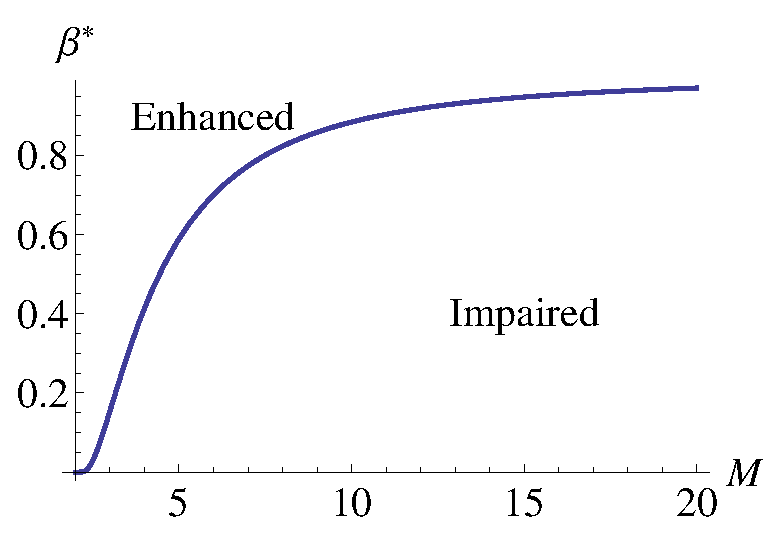
\includegraphics[width=0.45\linewidth]{multistate_betastar.eps}}\label{fig:multistate_betastar}
  \item\aligntop{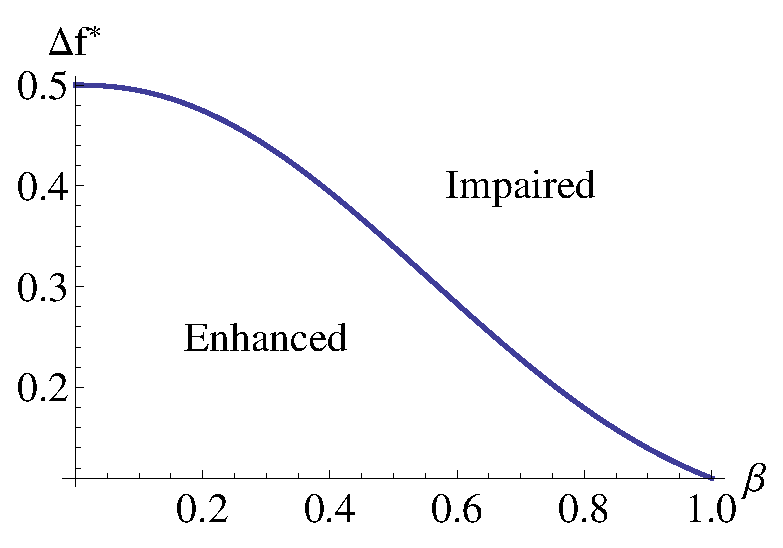
\includegraphics[width=0.45\linewidth]{multistate_deltafstar.eps}}\label{fig:multistate_deltafstar}
 \end{myenuma}
 \end{center}
  \caption[The functions $\beta^*(M)$ and $\Delta f^*(\beta,M)$]{The functions (\ref{fig:multistate_betastar}) $\beta^*(M)$, which describes when the \KO\ models have impaired learning, and (\ref{fig:multistate_deltafstar}) $\Delta f^*(\beta,M)$ for $M=10$, which describes when pre-training enhances learning.}\label{fig:multistate_star}
\end{figure}

In conclusion, if we choose $\beta<\beta^*(M)$, $\Delta f \in [\Delta f^*(1,M),\Delta f^*(\beta,M)]$, we will see that the \KO\ models learn slower than wild-type without pre-training, and that pre-training speeds up learning in the \KO\ models but slows it down in the wild-type.
%However, in this case pre-training proceeds much faster in the \KO\ models than wild-type (see \autoref{fig:multistate_med}\ref{fig:multistate_med_learn} and \autoref{fig:multistate_strong}\ref{fig:multistate_strong_learn}, lower curves), which is \emph{not} seen in the experiment.

%Now consider what would happen if we did not treat gain-increase and gain-decrease symmetrically.
%Let us set $f\pot\dec = f\pot\norm - \overline{\Delta f}$.
%Then, \eqref{eq:multiKOpre} becomes
%%
%\begin{equation}\label{eq:multiKOdiffpre}
%\begin{aligned}
%  \Phi &= 2\prn{\Delta f + \overline{\Delta f}} q \, \frac{(1-2\overline{\Delta f}) - \beta(1+2\overline{\Delta f})}
%          {(1-2\overline{\Delta f})^M - \beta^M(1+2\overline{\Delta f})^M}   \,
%          \brk{\beta (1-2\overline{\Delta f}) (1+2\overline{\Delta f})}^{M/2-1} \\
%       &= 2\prn{\Delta f + \overline{\Delta f}} q\,\frac{(1-\beta)\beta^{M/2-1}}{1-\beta^M} + \CO(\Delta f,\overline{\Delta f})^2.
%\end{aligned}
%\end{equation}
%%
%We can then look at the wild-type by setting $\beta=1$:
%%
%\begin{equation}\label{eq:multiWTdiffpre}
%\begin{aligned}
%  \Phi &= 8\,\overline{\Delta f}\prn{\Delta f + \overline{\Delta f}} q \,
%          \frac{(1-2\overline{\Delta f})^{M/2-1} (1+2\overline{\Delta f})^{M/2-1} }
%          {{(1+2\overline{\Delta f})^M - (1-2\overline{\Delta f})^M}}   \\
%       &= \frac{2\prn{\Delta f + \overline{\Delta f}} q}{M} + \CO(\Delta f,\overline{\Delta f})^2.
%\end{aligned}
%\end{equation}
%%
%
%We can see from these formulae that, if we want pre-training to impair learning in wild-type, but enhance it in the \KO\ models, the important thing is to have \emph{strong pre-training}, not strong training.
%Thus, removing the symmetry between gain-increase and gain-decrease will not help with the most unrealistic feature of this model -- the fact that pre-training proceeds much faster in the \KO\ models than wild-type.

%Finally, we note that, in the case of medium or strong pre-training, we see positive curvature in the learning curve after pre-training for a longer time in wild-type than in the \KO\ models (see \autoref{fig:multistate_med}\ref{fig:multistate_med_learnS} and \autoref{fig:multistate_strong}\ref{fig:multistate_strong_learnS}, dashed curves).
%This is due to the mass of probability at the right end of the chain
%%(see \autoref{fig:multistate_med}\ref{fig:multistate_med_eq} and \autoref{fig:multistate_strong}\ref{fig:multistate_strong_eq}, red trace)
%that is unable to contribute to change in synaptic weight until it has drifted to the centre.
%This will last for a shorter time in the \KO\ models, due to the enhanced transitions.
%This will not be a feature of any of the other models that we study here.
%Now, the curvature can be changed by the nonlinear relation between synaptic weight and VOR gain, but both curves would be affected in the same way.
%The difference in these two curvatures is therefore a good feature of this model.

%%%%%%%%%%%%%%%%%%%%%%%%%%%%%%%%%%%%%%%%%%%%%%%%%%%%%%%%%%%%%%%%%%%%%%%%%%



\subsection{Two-state model}\label{sec:binary}


%\resultsfign{two-state model}{binary}


The results of simulations of the two-state model can be seen in
\autoref{fig:sim_results}\ref{fig:binary_sim}.
%\autoref{fig:binary}.
However, this model can be solved exactly:
%
\begin{multline}\label{eq:binarysol}
  \eq = \frac{(f\dep q\dep, f\pot q\pot)}{\lambda},
  \qquad
  \pr(t) = \eq + (\pr(0)-\eq)\e^{-\lambda rt},\\
  \qquad \text{where} \quad
  \lambda = f\pot q\pot + f\dep q\dep.
\end{multline}
%
In practice, it is easier to just substitute $M=2$ into the formulae in \autoref{sec:multistate}.
%In this case, the initial rate of change and the total change encapsulate the whole solution, as there is only a single exponential decay.

We find that
%
\begin{equation}\label{eq:binaryflux}
  \Phi = \frac{q\pot q\dep \Delta f}{\lambda}, \qquad
  \pdiff{\Phi}{q\dep} = \frac{f\pot (q\pot)^2 \Delta f}{\lambda^2}, \qquad
  \pdiff{\Phi}{f\pot} = \frac{q\pot q\dep \lambda\inc}{\lambda^2}.
\end{equation}
%
The flux is a monotonically increasing function of $q\dep$ and $f\pot$.
Therefore, enhancing plasticity in this way, or pre-training, can only enhance the initial learning rate for all values of the parameters, unlike the experimental results shown in \modelfig.



We have only looked at the initial learning rate here, but for the experiments we looked at the learning after a finite period of time.
As the total change will be larger for the wild-type than \KO\ models, it must overtake eventually.
If this happens early enough (\ie between the first and second data point in \datafig), the initial period where the \KO\ models learns faster than wild-type would not be seen in the experiment.
However, the timescale for this crossover would be similar to the timescale of the exponentials, which is at least as long as the timescale for saturation of learning.
In \datafig\ we see that this timescale is longer than the gaps between successive measurements, so we would not miss any initial period of enhanced learning in the \KO\ mice if this were the correct model.
In addition, the models without pre-training can never catch up with those with pre-training, and this is sufficient to rule out this model.

This assumed that all synapses have the same parameters.
What would happen if there were a population of synapses with different parameters?
In this case, the learning rate would be determined by the average flux over this distribution:
%
\begin{equation}\label{eq:meanflux}
  \overline{\Phi} = \int \Phi(q\dep, \ldots) \,
                            p(q\dep, \ldots) \,
                          \dr q\dep \ldots,
\end{equation}
%
where the dependence on all other parameters is omitted.

The \KO\ mice will have a different distribution, $p\ko(q\dep, \ldots)$.
It is helpful to introduce a function $P(q\dep, \ldots)$ that is a cumulative distribution \wrt $q\dep$, but a probability density \wrt all other parameters:
%
\begin{equation}\label{eq:cumul}
  P(q\dep, \ldots) = \int_0^{q\pot} \!\!\! p(q, \ldots) \, \dr q.
\end{equation}
%
Then, integration by parts leads to
%
\begin{equation}\label{eq:fluxcumul}
  \overline{\Phi} = \av{\Phi(1, \ldots)} -
             \int \pdiff{\Phi}{q\pot} \,
                            P(q\dep, \ldots) \,
                          \dr q\dep \ldots,
\end{equation}
%
where the first term is averaged over all the other omitted parameters and the partial derivative is positive for this model \eqref{eq:binaryflux}.

The statement that the \KO\ models have larger $q\dep$ than wild-type is now a statement about the distributions, with the \KO\ models having more density at larger values.
This is not a precise concept, but it will tend to lead to $P(q\dep, \ldots)$ being smaller for the \KO\ models than wild type, which makes the second term less negative and the average flux larger, in contradiction with the experimental results in \modelfig.

If $P\ko \leq P\wt$ at all parameter values and the marginal distribution for all other parameters is the same for both models, then $\overline{\Phi}\ko \geq \overline{\Phi}\wt$.
This is guaranteed if, for example, there is a one-to-one map between $q\dep$ for the two models, so that the cumulative distributions are the same at $q\dep\wt$ and $q\dep\ko = g(q\dep\wt)$ for some function $g(x) \geq x$.

If the dependence of the distribution on $q\dep$ is mixed with the other parameters in some complicated way, or if the edges of the distributions are very unusual, it could be possible for the enhanced plasticity models to have an impaired initial learning rate, but this seems contrived and unlikely.
A similar argument applies to the effect of pre-training and the distributions over $f\pot$.

The monotonicity shown above means that this model cannot reproduce the key qualitative features of the experiments outlined in \autoref{sec:results}, at least as for the initial learning rate.
%This can be illustrated by looking at a special case, where $q\pot = q\dep = q$ for the wild type, $f\dep_0 = \frac{1}{2}$, $f\dep\dec = \frac{1}{2} - \Delta f$ and $f\dep\inc = \frac{1}{2} - \Delta f$.
%
%First, consider the wild-type.
%Without pre-training:
%%
%\begin{equation}\label{eq:binWTnopre}
%  \Phi = {\Delta f}\, q.
%\end{equation}
%%
%With pre-training:
%%
%\begin{equation}\label{eq:binWTpre}
%\begin{aligned}
%  \Phi &= 2{\Delta f}\, q.
%\end{aligned}
%\end{equation}
%%
%So, we see that pre-training will speed up learning, unlike what is seen in the experiment.
%This can be seen in
%\autoref{fig:sim_results}\ref{fig:binary_sim} %\autoref{fig:binary}\ref{fig:binary_learnS}
%(black curves).
%
%Now, consider the \KO\ models, for which we define $\beta=q\pot/q\dep<1$, and $q\pot=q$.
%Without pre-training:
%%
%\begin{equation}\label{eq:binKOnopre}
%  \Phi = \frac{2{\Delta f}\, q}{1+\beta},
%\end{equation}
%%
%which is larger than \eqref{eq:binWTnopre} for all $\beta$, unlike what is seen in the experiments (see \modelfig).
%This is also seen in
%\autoref{fig:sim_results}\ref{fig:binary_sim} %\autoref{fig:binary}\ref{fig:binary_learn},\ref{fig:binary_learnS}
%(solid curves).
%As discussed above (below \eqref{eq:multiKOnopre}), the larger value of $q\dep=q/\beta$ has two effects.
%Smaller $\beta$ will increase the probability of depression, speeding up learning, but it will also decrease the probability of being ready for depression, slowing down learning.
%For the serial model, we argued that the first effect goes like $1/\beta$, whereas the second goes like $\beta^{M/2}$ to leading order.
%Here $M=2$, so the leading part of the two effects will cancel.
%The subleading effects (the normalisation of the probabilities) are responsible for the faster learning in the \KO\ models.
%
%%With pre-training:
%%%
%%\begin{equation}\label{eq:binKOpre}
%%\begin{aligned}
%%  \Phi &= 4{\Delta f}\, q \, \frac{(1-2\Delta f) - \beta(1+2\Delta f)}
%%          {(1-2\Delta f)^2 - \beta^2(1+2\Delta f)^2}.
%%\end{aligned}
%%\end{equation}
%%%
%%As we've already ruled out this model, we will not analyse this formula any further.
%As this model is already ruled out, we will not analyse pre-training in the \KO\ models.


For this simple binary synapse model, the ratio of the numbers of potentiated and depressed synapses is equal to the ratio of the potentiating and depressing transition rates.
This means that the leading effects of enhanced intrinsic plasticity rates and saturation bias cancel each other.
This is even true as the number of synapses available for further plasticity approaches zero, which requires that the depressing transition be infinitely stronger than the potentiating transition, compensating for the saturation.
There is a requirement that the total number of synapses, potentiated and depressed, is fixed.
This normalization effect dampens the effect of saturation bias, so that the effect of enhanced intrinsic plasticity rates dominates for all parameter values.
Thus, we must see enhanced initial learning with enhanced plasticity in the binary synapse model.

One can see that pre-training can only increase the fraction of synapses available for depression.
This model has no mechanism that could ever result in this causing impaired learning.

Intuitively, this model is missing two features of the \hyperref[sec:multistate]{serial model}.
First, it does not have the exponential amplification of the effect of initial saturation bias because this model does not have a chain of states for the distribution to decay across.
Second, it does not have the metaplastic effect where repeated potentiation makes future depression harder, as potentiation will merely increase the number of potentiated synapses.


%%%%%%%%%%%%%%%%%%%%%%%%%%%%%%%%%%%%%%%%%%%%%%%%%%%%%%%%%%%%%%%%%%%%%%%%%%


\subsection{Multistate model}\label{sec:multistate_lin}

%\resultsfign{multistate model}{multistate_lin}


In this section, we will consider the multistate model as defined in \cite{amit1994learning}, \ie with linearly varying synaptic weight.
The numerical results can be seen in
\autoref{fig:sim_results}\ref{fig:multistate_sim}, %\autoref{fig:multistate_lin},
but we can get some analytic insight into this model as well.
In essence, this model is like a series of two-state models attached to each other, in contrast to the serial model for which the synaptic weight only changes between one of the pairs of states.


The equilibrium distribution, \eqref{eq:mutltieq}, still applies.
However, now the rate of change of our learning metric, \eqref{eq:learning}, will be proportional to the sum of the net fluxes between adjacent states:
%
\begin{equation}\label{eq:multiLinFlux}
  \begin{aligned}
    \Phi &= \sum_{i=1}^{M-1} \eq_{i+1} f'{}\dep q\dep - \eq_i f'{}\pot q\pot
         %&= \sum_{i=1}^{M-1} \eq_i (\alpha-\alpha') f'{}\dep q\dep \\
         &= \frac{1-\alpha^{M-1}}{1-\alpha^M} \, \prn{\frac{\alpha}{\alpha\inc}} f\inc\pot q\pot.
  \end{aligned}
\end{equation}
%

To see the effects of the knockout, we can see if this increases or decreases with $q\dep$:
%
\begin{equation}\label{eq:multiderq}
  q\dep \pdiff{\Phi}{q\dep} =
    \frac{\alpha^{M - 1}}{(1 - \alpha^M)^2}
    \brk{1 - \alpha}
    \brk{M - \sum_{i=1}^M \alpha^{i-1}}
    \prn{\frac{\alpha}{\alpha\inc} - 1} f\inc\pot  q\pot.
\end{equation}
%
If $\alpha < 1$, both quantities in square brackets are positive, as the sum contains $M$ terms that are all at most $1$.
If $\alpha > 1$, both of them are negative.
Therefore this quantity is positive, so $\Phi$ is a monotonically increasing function of $q\dep$.
Therefore, enhancing plasticity in this way can only enhance the initial learning rate, for all values of the parameters.

We can also see the effects of pre-training on the initial learning rate by seeing if it increases or decreases with $f\pot$ (with $f\dep = 1 - f\pot$):
%
\begin{equation}\label{eq:multiderf}
  f\pot f\dep \pdiff{\Phi}{f\pot} =
    \frac{\alpha^{M - 2}}{(1 - \alpha^M)^2}
      \brk{1 - \alpha}
      \prn{\brk{M - \sum_{i=1}^M \alpha^{i-1}}
      + \frac{\alpha}{\alpha\inc} \brk{\sum_{i=1}^M \alpha^{1-i} - M}}
      f\inc\pot  q\pot.
\end{equation}
%
This quantity is positive, for similar reasons to \eqref{eq:multiderq}, so $\Phi$ is a monotonically increasing function of $f\pot$.
Therefore, pre-training can can only enhance the initial learning rate, for all values of the parameters.

The monotonicity shown above means that this model cannot reproduce the key qualitative features of the experiments outlined in \autoref{sec:results}, at least as for the initial learning rate.
%This can be illustrated by looking at a special case, where $q\pot = q\dep = q$ for the wild type, $f\dep_0 = \frac{1}{2}$, $f\dep\dec = \frac{1}{2} - \Delta f$ and $f\dep\inc = \frac{1}{2} - \Delta f$.
%
%First, consider the wild-type, for which $q\pot=q\dep=q$.
%Without pre-training:
%%
%\begin{equation}\label{eq:multiLinWTnopre}
%  \Phi = 2{\Delta f}\,q\,\frac{M-1}{M}.
%\end{equation}
%%
%With pre-training:
%%
%\begin{equation}\label{eq:multiLinWTpre}
%\begin{aligned}
%  \Phi &= 4{\Delta f}\, q \, \frac{(1+2\Delta f)^{M-1} - (1-2\Delta f)^{M-1}}
%          {(1+2\Delta f)^M - (1-2\Delta f)^M} \\
%       &= {4{\Delta f}\, q}\,\frac{M-1}{M} + \CO(\Delta f)^2.
%\end{aligned}
%\end{equation}
%%
%
%Now, consider the \KO\ models, for which we define $\beta=q\pot/q\dep<1$, and we set $q\pot=q$.
%Without pre-training:
%%
%\begin{equation}\label{eq:multiLinKOnopre}
%  \Phi = 2{\Delta f}\, q\,\frac{1-\beta^{M-1}}{1-\beta^M}.
%\end{equation}
%%
%This decreases monotonically in the interval $\beta\in[0,1]$, therefore this will always be greater than \eqref{eq:multiLinWTnopre}.
%This means that the \KO\ models will initially learn faster than the wild-type.
%However the wild-type will eventually catch up, and this can happen very quickly, as seen in
%\autoref{fig:sim_results}\ref{fig:multistate_sim} %\autoref{fig:multistate_lin}\ref{fig:multistate_lin_learn},\ref{fig:multistate_lin_learnS}
%(solid curves).
%
%With pre-training:
%%
%\begin{equation}\label{eq:multiLinKOpre}
%\begin{aligned}
%  \Phi &= 4{\Delta f}\, q \, \frac{(1-2\Delta f)^{M-1} - \beta^{M-1}(1+2\Delta f)^{M-1}}
%          {(1-2\Delta f)^M - \beta^M(1+2\Delta f)^M} \\
%       &= 4{\Delta f}\, q\,\frac{1-\beta^{M-1}}{1-\beta^M} + \CO(\Delta f)^2.
%\end{aligned}
%\end{equation}
%%
%The ratio of this to \eqref{eq:multiLinKOnopre} takes its minimum value at the upper end of the interval $\Delta f \in \brk{0,\half}$, where it takes the value
%%
%\begin{equation}\label{eq:multiLinprenopre}
%  \frac{\Phi_{\text{w/ pre}}}{\Phi_{\text{w/o pre}}} = \frac{1-\beta^M}{\beta-\beta^M}
%   \longrightarrow \frac{M}{M-1} \quad \text{as} \quad \beta\to1,
%\end{equation}
%%
%which is always greater than 1.
%Therefore, pre-training will enhance the initial learning rate for all parameter values, for both \KO\ models and wild-type, as seen in
%\autoref{fig:sim_results}\ref{fig:multistate_sim}. %\autoref{fig:multistate_lin}\ref{fig:multistate_lin_learnS}.

We have only looked at the initial learning rate here, but for the experiments we looked at the learning after a finite period of time.
Just as the case of the  \hyperref[sec:binary]{two state model}, the wild-type will eventually catch up with \KO\ model.
This can happen very quickly, as seen in \autoref{fig:sim_results}\ref{fig:multistate_sim} (solid curves).
This means that the initial period, where the \KO\ models learns faster than wild-type, might not be seen in the experiment.
However, the models without pre-training can never catch up with those with pre-training, and this is sufficient to rule out this model.


Like the \hyperref[sec:binary]{two state model}, this model is missing two features of the \hyperref[sec:multistate]{serial model}.
First, it does not have the amplification of the effect of initial saturation bias as every transition contributes to the learning signal, so the exponentially decaying distribution has no effect.
Second, it does not have the metaplastic effect where repeated potentiation makes future depression harder, as potentiation will merely increase the number of potentiated synapses without pushing them away from any boundary between strong and weak states.



%%%%%%%%%%%%%%%%%%%%%%%%%%%%%%%%%%%%%%%%%%%%%%%%%%%%%%%%%%%%%%%%%%%%%%%%%%


\subsection{Pooled resource model}\label{sec:pooled}
%
%
%\resultsfig{pooled resource}{light depletion}{($q\lmin/q\lmax=0.75$)}{pooled_plenty}
%
%\resultsfig{pooled resource}{heavy depletion}{($q\lmin/q\lmax=0.125$)}{pooled_scarce}
%
%\resultsfign{pooled resource}{pooled_deponly}


The results of simulations of the pooled resource model can be seen in
\autoref{fig:sim_results}\ref{fig:pooled_sim}. %\autoref{fig:pooled_deponly}.
%It is difficult to study this model analytically.
%However, the numerical results can help us understand it qualitatively.
The numerical results can help us understand it qualitatively.

If we compare gain-increase learning in the \KO\ models to wild-type, there are two effects: the increased transition rates speed up learning, but the equilibrium distribution is shifted to the depressed side,
% (compare \autoref{fig:pooled_deponly}\ref{fig:pooled_deponly_eq}: \ref{fig:pooled_deponly_eq_WT} and \ref{fig:pooled_deponly_eq_KO}, blue traces),
where there are fewer synapses available for depression and resources are depleted.
When resource depletion is sufficiently severe, the second effect dominates and the \KO\ models learn slower than wild-type (see \autoref{fig:sim_results}\ref{fig:pooled_sim}, %\autoref{fig:pooled_deponly}\ref{fig:pooled_deponly_learn},\ref{fig:pooled_deponly_learnS},
solid curves), which matches what is seen in the experiment.

Gain-decrease pre-training lessens the second effect, and results in the \KO\ models learning faster than wild-type (see \autoref{fig:sim_results}\ref{fig:pooled_sim}, %\autoref{fig:pooled_deponly}\ref{fig:pooled_deponly_learn},\ref{fig:pooled_deponly_learnS}
red curves),
as seen in the experiment.

Gain-decrease pre-training will shift the distribution to the potentiated side, where there are more synapses available for depression and resources are more plentiful, for both the \KO\ models and wild type.
This means that the pre-trained animals will learn faster then the untrained one for both \KO\ models and wild-type (see \autoref{fig:sim_results}\ref{fig:pooled_sim}). %\autoref{fig:pooled_deponly}\ref{fig:pooled_deponly_learnS}).
This differs from what is seen experimentally, where the pre-trained wild-type learns slower than the untrained one.

\hypertarget{par:pooled_scan}{To} verify that this always happens, we scanned over acceptable values of the six parameters relevant to gain-decrease pre-training in wild-type models: $q\pot$, $q\dep\lmin < q\dep\lmax$, and $f\dep\dec < f\dep\norm < f\dep\inc$.
Each parameter was scanned over 10 values from 0.05 to 0.95, rejecting values that do not respect the inequalities above.
For each parameter set, we computed the initial learning rate, $\dot{L}(0)$ from \eqref{eq:learning}, with and without pre-training.
To qualitatively reproduce the experimental results, we would need $\dot{L}_\text{no pre} - \dot{L}_\text{pre} > 0$ at $t = 0$.
The range of values obtained is plotted in \autoref{fig:pooled_scan}, where we see that this difference is always negative, ruling out this model.

\begin{figure}
  \centering
  % Requires \usepackage{graphicx}
  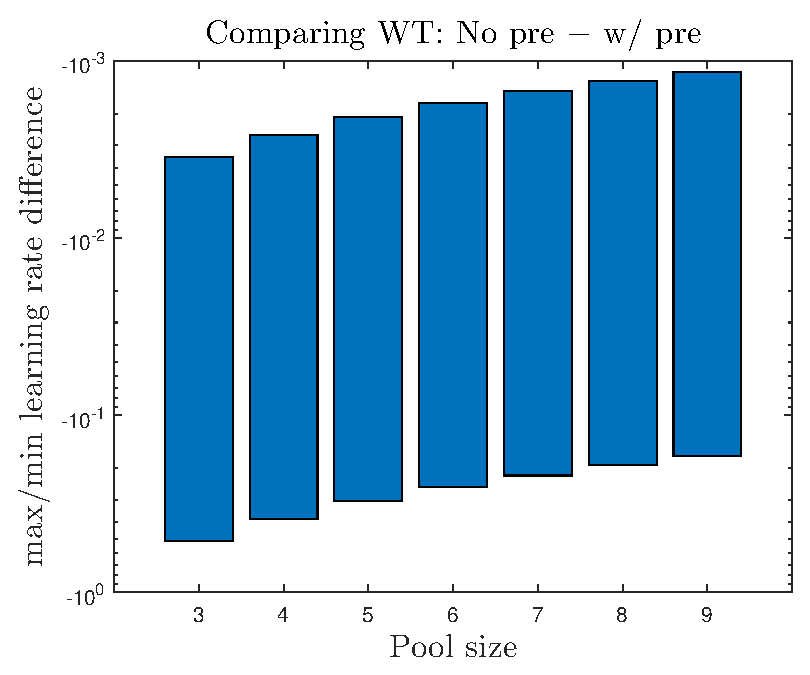
\includegraphics[width=0.4\linewidth]{pooled_deponly_scan.eps}
  \caption{Difference in initial learning rate in wild-type models, without and with gain-decrease pre-training.
  Learning, $L(t)$ is defined in \eqref{eq:learning}.
  Here, we show the maximum and minimum values of this quantity when scanning all 6 relevant parameters (see \protect\hyperlink{par:pooled_scan}{text}).
  We see that this quantity is always negative, whereas it was positive in the experiments.
  }\label{fig:pooled_scan}
\end{figure}


This model shares one feature of the \hyperref[sec:multistate]{serial model}.
The effect of initial saturation bias is amplified by resource depletion, allowing for impaired learning with enhanced plasticity.
However, it does not have the metaplastic effect where repeated potentiation makes future depression harder, in fact it shows the opposite effect due to resource replenishment, so it can never show impaired learning after pre-training.


%%%%%%%%%%%%%%%%%%%%%%%%%%%%%%%%%%%%%%%%%%%%%%%%%%%%%%%%%%%%%%%%%%%%%%%%%%


\subsection{Cascade and non-uniform multistate models}\label{sec:cascade}

%\resultsfig{cascade}{short pre-training}{($rt_\text{pre}=20$)}{cascade_short}
%
%\resultsfig{cascade}{long pre-training}{($rt_\text{pre}=100$)}{cascade_long}



The results of simulations of the cascade and non-uniform multistate models can be seen in
\autoref{fig:sim_results}\ref{fig:cascade_sim},\ref{fig:nonuni_sim}. %\autoref{fig:cascade_short} and \autoref{fig:cascade_long}.
%It is difficult to study these models analytically.
%However, the numerical results can help us understand them qualitatively.
The numerical results can help us understand them qualitatively.

For the cascade model, we see that the \KO\ models are slower than wild-type without pre-training but faster with it.
This seems to be due to the fact that, without pre-training, very few synapses will be available for depression as most of them are already depressed.
%(\autoref{fig:cascade_short}\ref{fig:cascade_short_eq}\ref{fig:cascade_short_eq_KO} and \ref{fig:cascade_short_pr}\ref{fig:cascade_short_pr_KO_nopre}).
With pre-training, some of them will now be potentiated,
%(\autoref{fig:cascade_short}\ref{fig:cascade_short_eq}\ref{fig:cascade_short_eq_KO} and \ref{fig:cascade_short_pr}\ref{fig:cascade_short_pr_KO_pre}),
and the enhanced depression can speed up learning.

%With shorter pre-training, we see that it speeds up learning in both wild-type and \KO\ models (see \autoref{fig:cascade_short}\ref{fig:cascade_short_learnS}), whereas experimentally this only happens for the \KO\ models.
%This is due to the fact that pre-training results in more synapses being potentiated, and thus ready for depression, but does not push them far enough down the cascade for the lower transition probabilities to slow down learning (see \autoref{fig:cascade_short}\ref{fig:cascade_short_pr}\ref{fig:cascade_short_pr_WT_pre}).
%
%We can see from \autoref{fig:cascade_long}\ref{fig:cascade_long_pr}\ref{fig:cascade_long_pr_WT_pre} that longer

Sufficiently long pre-training pushes the synapses far down the cascade, slowing down learning for the wild-type (see \autoref{fig:sim_results}\ref{fig:cascade_sim}, black curves).
This effect is weaker for the \KO\ models, as the equilibrium distribution is not as heavily concentrated at the end, as the distribution before pre-training is shifted in the opposite direction.
%(see \autoref{fig:cascade_long}\ref{fig:cascade_long_eq}\ref{fig:cascade_long_eq_KO}).


For the non-uniform multistate model, we see that the \KO\ models are slower than wild-type without pre-training, as seen experimentally.
This seems to be because the enhanced depression results in a greater fraction of synapses begin in states of weaker synaptic weight %(see \autoref{fig:nonuni}\ref{fig:nonuni_eq}\ref{fig:nonuni_eq_KO})
where the depressing transitions have lower probability (see \autoref{fig:models}\ref{fig:nonuni_model}).

However, gain-decrease pre-training will push synapses towards the states of stronger synaptic weight.
The wild-type will be pushed further that the \KO\ models, as the latter started further to the weaker side as explained above. %(compare \autoref{fig:nonuni}\ref{fig:nonuni_eq}\ref{fig:nonuni_eq_WT} and \ref{fig:nonuni_eq_KO}).
As the depressing transitions have lower probability for the strongest states (see \autoref{fig:models}\ref{fig:nonuni_model}), this, in addition to the enhanced depression of the \KO\ models, will result in the \KO\ models learning faster than wild-type, as seen experimentally.

When comparing learning with and without gain-decrease pre-training, there are two effects to consider.
First, the synapses are pushing towards the states of stronger synaptic weight, resulting in more synapses being available for depression, speeding up learning.
Second, it will also place synapses in states where transitions have lower probability, slowing down learning.
The second effect will be weaker in the \KO\ models than in wild-type, as they started further to the weaker side as explained above.
This means that, for appropriate parameter choices, gain-decrease pre-training can speed up learning in the \KO\ models, but also slow down learning in wild-type, as seen experimentally.

These models share both key features of the \hyperref[sec:multistate]{serial model}.
First, the effect of initial saturation bias is amplified by the exponential decay of transition probabilities away from the middle.
Second, they both have the metaplastic effect where repeated potentiation makes future depression harder, also due to he exponential decay of transition probabilities.


%\subsection{Non-uniform multistate model}\label{sec:nonuni}
%
%%\resultsfign{non-uniform multistate}{nonuni}
%
%
%
%The results of simulations of the non-uniform multistate model can be seen in
%\autoref{fig:sim_results}\ref{fig:nonuni_sim}. %\autoref{fig:nonuni}.
%It is difficult to study this model analytically.
%However, the numerical results can helps us understand it qualitatively.
%
%First, we see that the \KO\ models are slower than wild-type without pre-training, as seen experimentally.
%This seems to be because the enhanced depression results in a greater fraction of synapses begin in states of weaker synaptic weight %(see \autoref{fig:nonuni}\ref{fig:nonuni_eq}\ref{fig:nonuni_eq_KO})
%where the depressing transitions have lower probability (see \autoref{fig:nonuni_model}).
%
%However, gain-decrease pre-training will push synapses towards the states of stronger synaptic weight.
%The wild-type will be pushed further that the \KO\ models, as the latter started further to the weaker side as explained above. %(compare \autoref{fig:nonuni}\ref{fig:nonuni_eq}\ref{fig:nonuni_eq_WT} and \ref{fig:nonuni_eq_KO}).
%As the depressing transitions have lower probability for the strongest states (see \autoref{fig:nonuni_model}), this, in addition to the enhanced depression of the \KO\ models, will result in the \KO\ models learning faster than wild-type, as seen experimentally.
%
%When comparing learning with and without gain-decrease pre-training, there are two effects to consider.
%First, the pushing synapses towards the states of stronger synaptic weight, resulting in more synapses being available for depression, speeding up learning.
%Second, it will also place synapses in states where transitions have lower probability, slowing down learning.
%The second effect will be weaker in the \KO\ models than in wild-type, as they started further to the weaker side as explained above.
%This means that, for appropriate parameter choices, gain-decrease pre-training can speed up learning in the \KO\ models, but also slow down learning in wild-type, as seen experimentally.
%
%Like the \hyperref[sec:cascade]{cascade model}, this model also shares both features of the \hyperref[sec:multistate]{serial model}.
%First, the effect of initial saturation bias is amplified by the exponential decay of transition probabilities away from the middle.
%Second, it has the metaplastic effect where repeated potentiation makes future depression harder, also due to he exponential decay of transition probabilities.



%\subsection{Parameter fitting}\label{sec:fit}
%
%So far, we have only considered the comparisons listed at the start of \hyperref[sec:results]{this section}, as they raised important conceptual questions.
%We have not considered the other two comparisons, the lack of difference between wild-type without pre-training and \KO\ with pre-training and between wild-type with pre-training and \KO\ without pre-training (the ``diagonal'' comparisons in the language of \modelfig), as they depend more on the values used for the parameters than on any conceptual issues.
%
%However, to avoid confusion, we found parameter values performed reasonably in these other two comparisons for the three models that could reproduce the correct qualitative results of the four important comparisons: the \hyperref[sec:multistate]{serial model}, the \hyperref[sec:cascade]{cascade model} and the \hyperref[sec:nonuni]{non-uniform multistate model}. The learning curves are shown in \autoref{fig:fit} and the parameters are listed in \autoref{fig:fit}\ref{tab:fit}.
%
%
%%\begin{table}
%% \begin{center}
%%  \begin{tabularn}{|l|c|c|c|c|c|c|c|c|c|}
%%    \cline{1-10}
%%    % after \\: \hline or \cline{col1-col2} \cline{col3-col4} ...
%%    Model & \# states & \multicolumn{3}{c|}{parameter} & \multicolumn{3}{c|}{$f\dep$} & \multicolumn{2}{c|}{$rt$} \\
%%    \cline{3-10}
%%    & & pot & WT dep & \KO\ dep & base & inc & dec & train & pre \\
%%
%%    \cline{1-10}
%%    Serial   & 10 & $0.12$  & $0.14$  & $0.2$  & 0.5 & 0.11 & 0.89 & 5  & 100  &\label{tr:serial_fit} \\
%%    Cascade  & 14 & $0.386$  & $0.398$  & $0.466$  & 0.522 & 0.63 & 0.002 & 1.5  & 200  &\label{tr:cascade_fit} \\
%%    Non-uni. & 12 & $0.4$    & $0.4$    & $0.53$   & 0.5 & 0.7 & 0.1 & 5  & 500  &\label{tr:nonuni_fit} \\
%%    \cline{1-10}
%%  \end{tabularn}
%% \end{center}
%%  \caption{Parameters used to reproduce detailed experimental results. For the sewrial model, the parameter listed is the transition probability between adjacent states. For the cascade and non-uniform multistate models, the parameter is the ratio of adjacent transition probabilities.} \label{tab:fit}
%%\end{table}
%
%\begin{figure}
% \begin{center}
% \begin{myenuma}
%  \item\aligntop{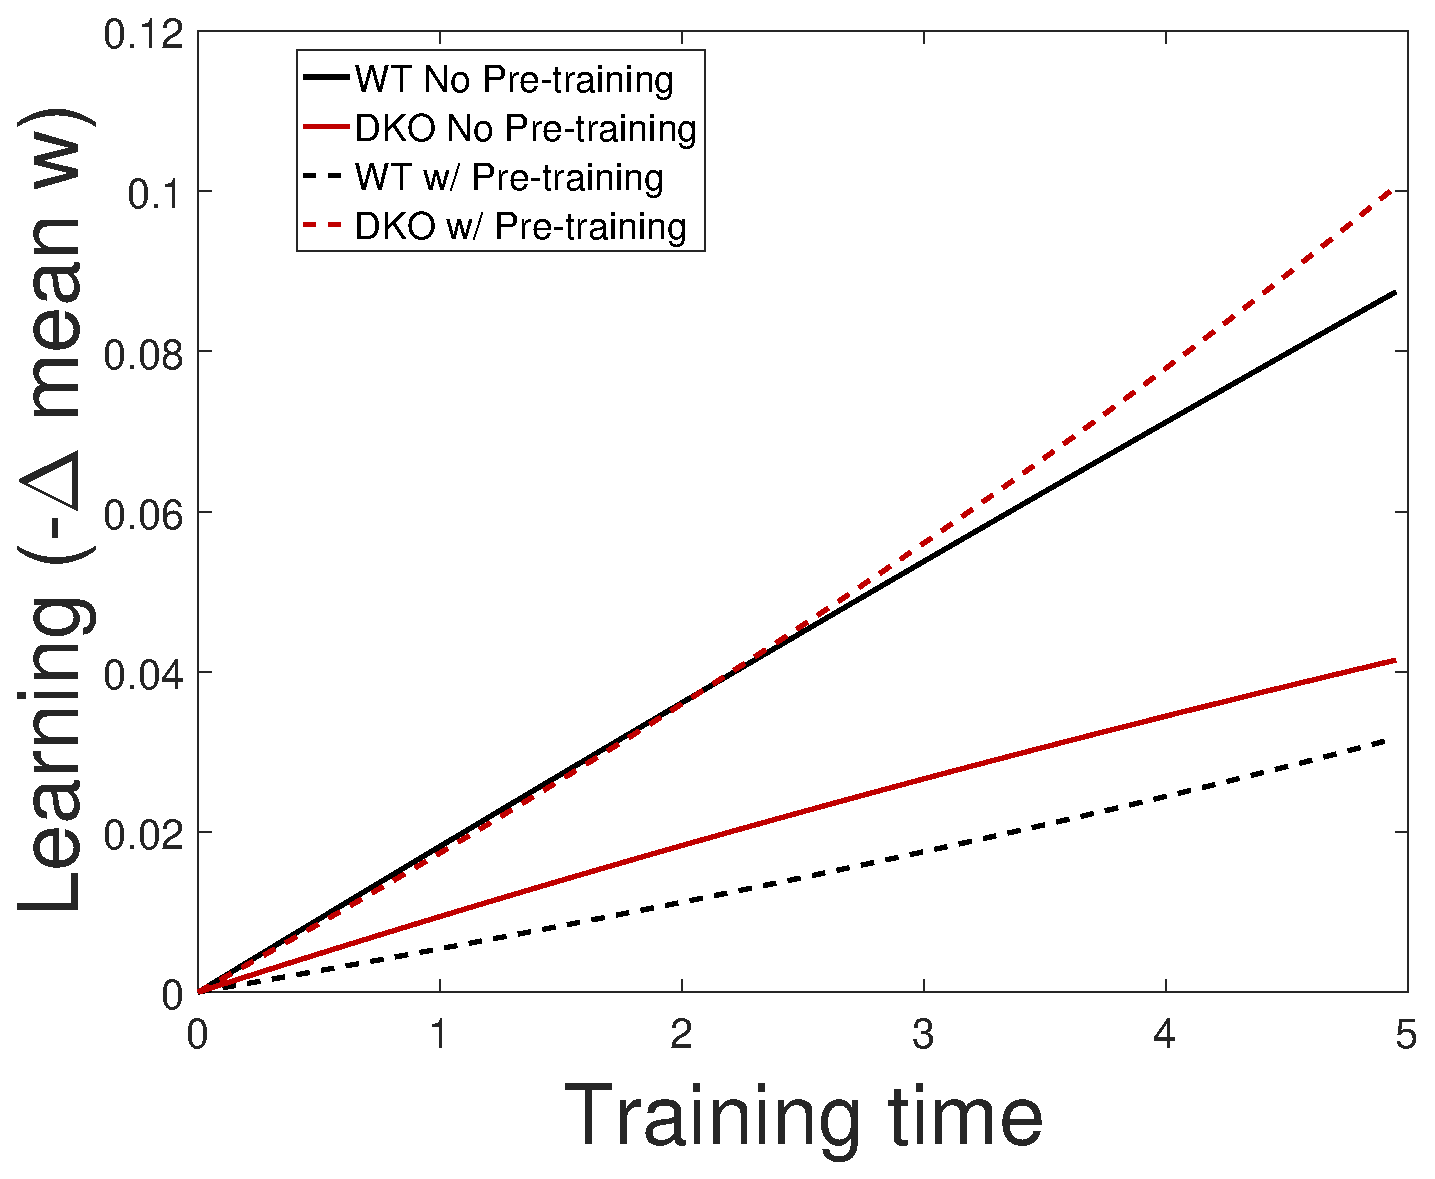
\includegraphics[width=0.28\linewidth]{serial_fit_learnS.eps}}\label{fig:serial_fit}
%  \item\aligntop{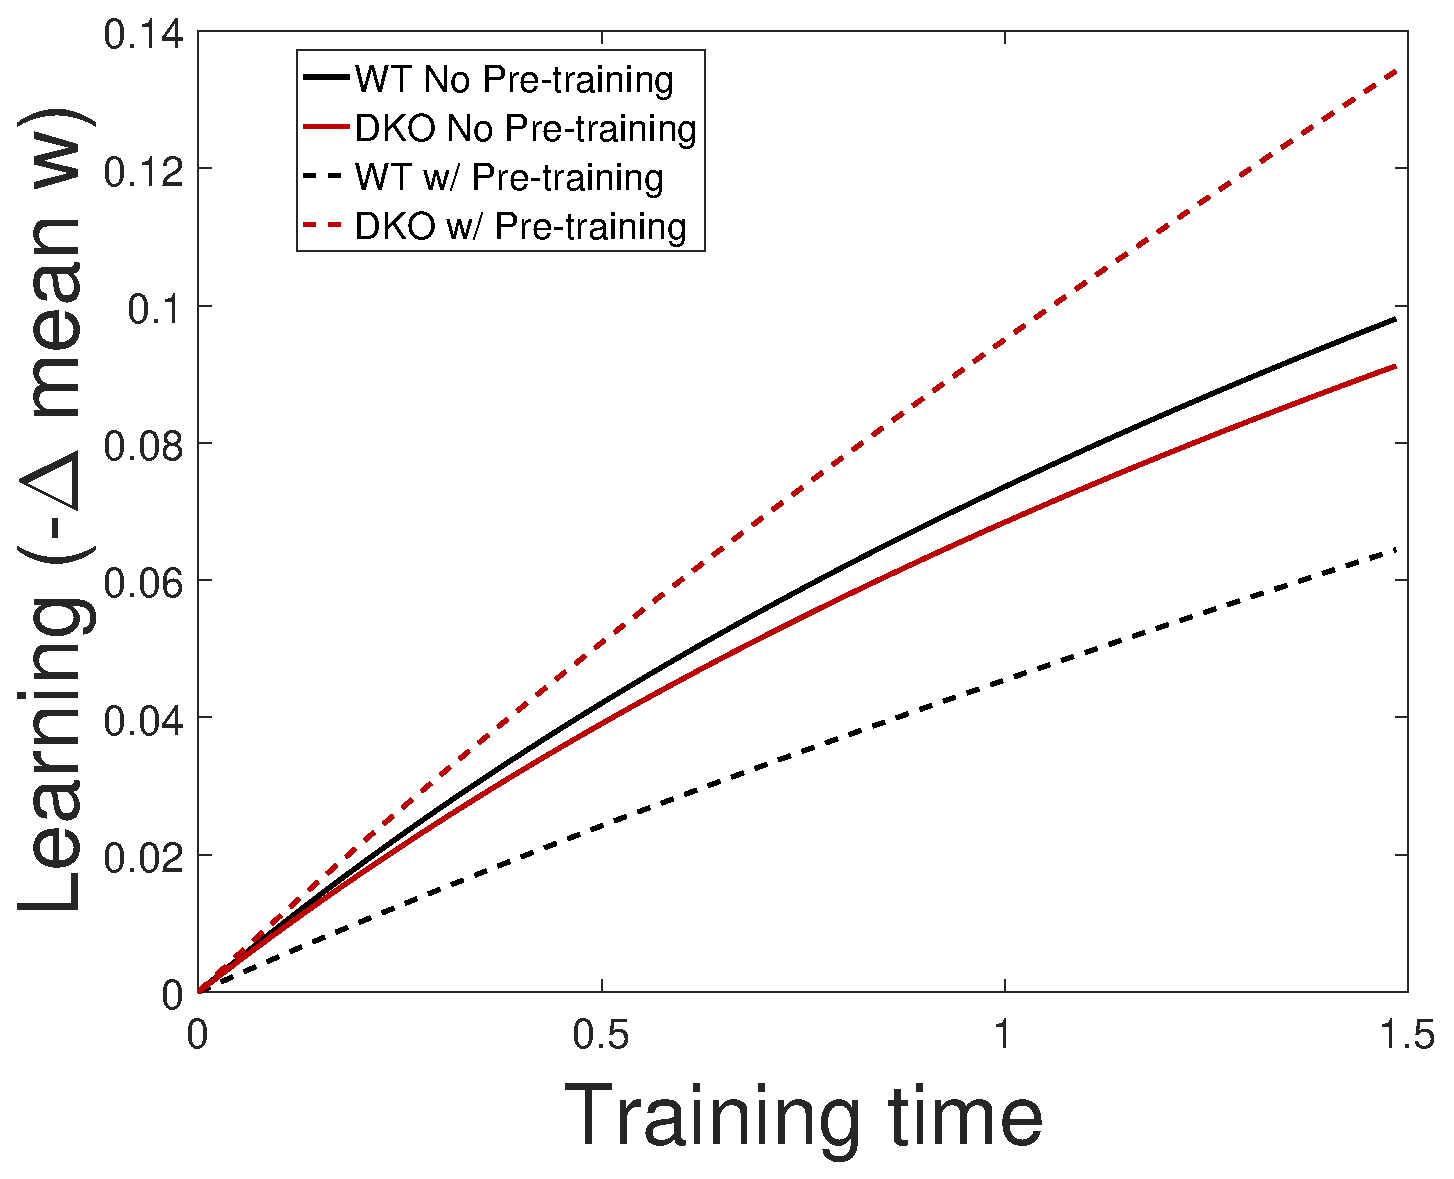
\includegraphics[width=0.28\linewidth]{cascade_fit_learnS.eps}}\label{fig:cascade_fit}
%  \item\aligntop{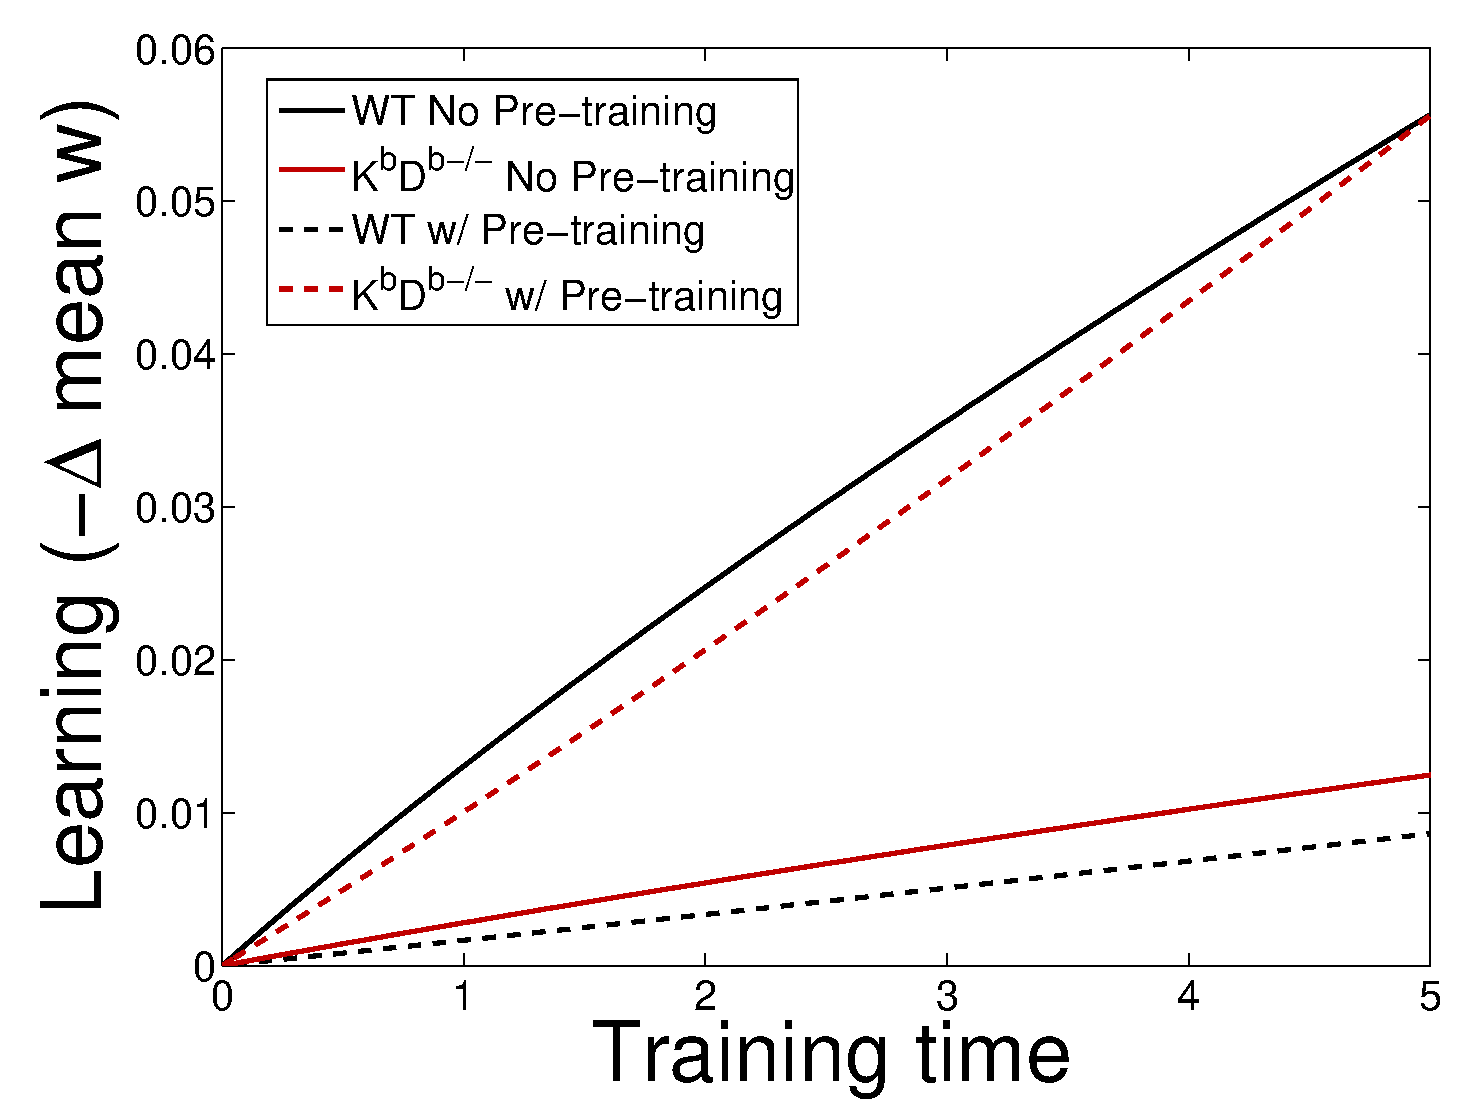
\includegraphics[width=0.28\linewidth]{nonuni_fit_learnS.eps}}\label{fig:nonuni_fit}
%
%  \vspace{1cm}\item\label{tab:fit}\aligntop{
%  \begin{tabularn}{|l|c|c|c|c|c|c|c|c|}
%    \cline{1-9}
%    % after \\: \hline or \cline{col1-col2} \cline{col3-col4} ...
%    Model & \#  & \multicolumn{3}{c|}{parameter} & \multicolumn{3}{c|}{$f\dep$} & $r\tpre$ \\
%    \cline{3-8}
%    & states & pot & WT dep & {\footnotesize\KO} dep & base & inc & dec &  \\
%
%    \cline{1-9}
%    Serial   & 10 & $0.12$  & $0.14$  & $0.2$  & 0.5 & 0.89 & 0.11  & 100  &\label{tr:serial_fit} \\
%    Two-state     & 2  & $0.1$  & $0.1$  & $0.2$  & 0.5 & 0.6 & 0.4  & 5   &\label{tr:binary} \\
%    Multistate    & 10 & $0.3$  & $0.3$  & $0.4$  & 0.5 & 0.8 & 0.2  & 5   &\label{tr:multistate_lin} \\
%    Pooled res. & 7  & $0.008$        & $[0.0006,0.6]$  & $[0.001,1]$
%                                          & 0.5 & 0.9 & 0.1 & 20 &\label{tr:pooled_deponly}\\
%    Cascade  & 14 & $0.386$  & $0.398$  & $0.466$  & 0.522 & 0.63 & 0.002  & 200  &\label{tr:cascade_fit} \\
%    Non-uni. & 12 & $0.4$    & $0.4$    & $0.53$   & 0.5 & 0.7 & 0.1 & 500  &\label{tr:nonuni_fit} \\
%    \cline{1-9}
%  \end{tabularn}}
% \end{myenuma}
% \end{center}
%  \caption[Learning curves for models after parameter fitting]{Learning curves restricted to gain-increase training, for (\ref{fig:serial_fit}) the serial model, (\ref{fig:cascade_fit}) the cascade model, and (\ref{fig:nonuni_fit}) the non-uniform multistate model.
%  (\ref{tab:fit}) Parameters used to reproduce detailed experimental results. For the serial model, the parameter listed is the transition probability between adjacent states. For the cascade and non-uniform multistate models, the parameter is the ratio of adjacent transition probabilities.}\label{fig:fit}
%\end{figure}

%%%%%%%%%%%%%%%%%%%%%%%%%%%%%%%%%%%%%%%%%%%%%%%%%%%%%%%%%%%%%%%%%%%%%%%%%%


\section{Long term effects of pre-training}\label{sec:longterm}


The fact that after pre-training, gain-increase learning is significantly faster in the \KO\ models than in the wild-type, as discussed in the \hyperref[sec:results]{previous section}, is true of the initial learning rate.
With a long enough duration of training, memory of the initial conditions should be erased and the final learning outcome should be the same with or without pre-training.
In \autoref{fig:longterm} we show the result of longer training durations on the three models that were not ruled out on the basis of the initial learning rate, the serial, cascade and nonuniform multistate models.
For all of these models, we see that the wild-type models eventually catch up and overtake the \KO\.
The initial learning enhancement is a transient effect, and at later times it turns into a learning impairment.




\begin{figure}
  \centering
  \begin{myenuma}
  \item\aligntop{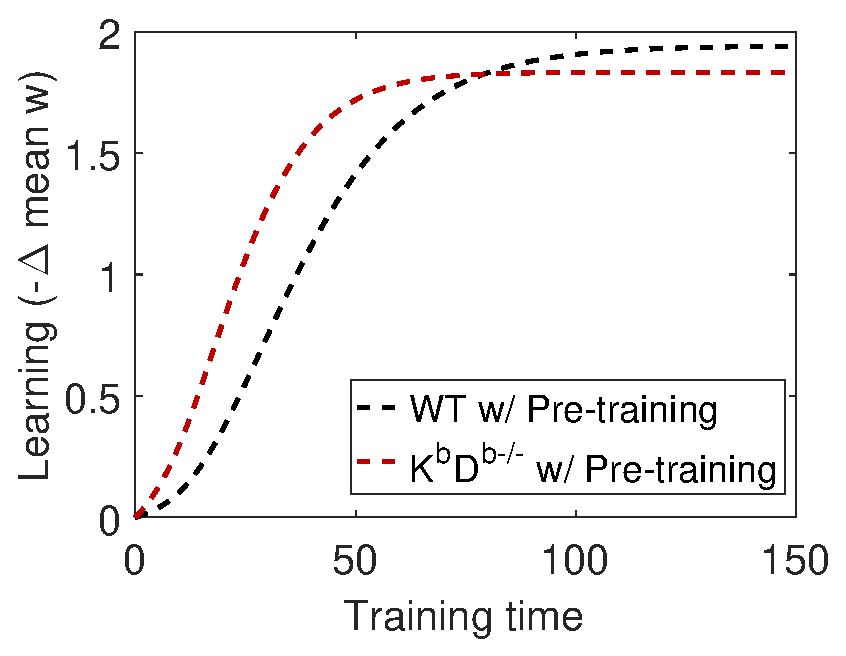
\includegraphics[width=0.29\linewidth]{serial_longterm.eps}}\label{fig:serial_longterm}
  \item\aligntop{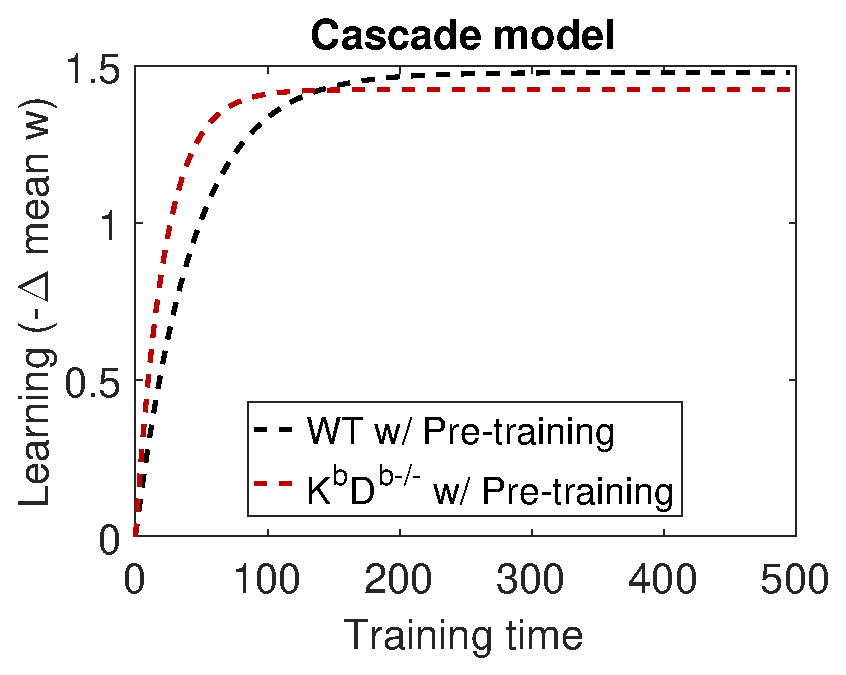
\includegraphics[width=0.29\linewidth]{cascade_longterm.eps}}\label{fig:cascade_longterm}
  \item\aligntop{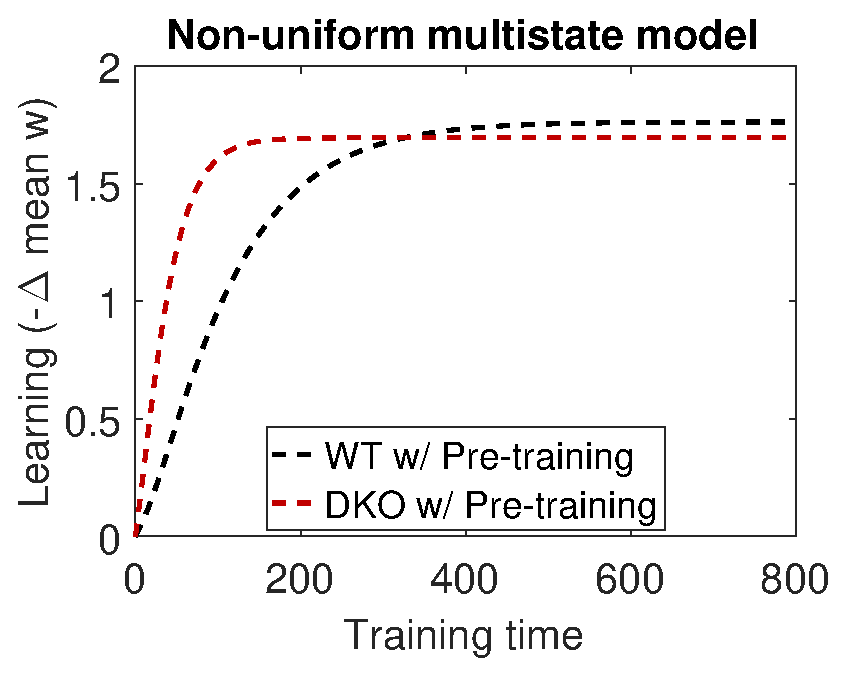
\includegraphics[width=0.29\linewidth]{nonuni_longterm.eps}}\label{fig:nonuni_longterm}
  \end{myenuma}
  \caption{ Simulation of training for long times after pre-training shows that it erases the effect of pre-training.
  These simulations were performed with the same parameters as in \autoref{fig:sim_results}\ref{tab:params}, but with much longer training times, for the (\ref{fig:serial_longterm}) serial, (\ref{fig:cascade_longterm} cascade and (\ref{fig:nonuni_longterm}) non-uniform multistate models.
  Compare with \autoref{fig:sim_results}\ref{fig:serial_sim},\ref{fig:cascade_sim},\ref{fig:nonuni_sim}.
  }\label{fig:longterm}
\end{figure}





%%%%%%%%%%%%%%%%%%%%%%%%%%%%%%%%%%%%%%%%%%%%%%%%%%%%%%%%%%%%%%%%%%%%%%%%%%


\section{Model of non-specific CF stimulation}\label{sec:chr2}

\begin{figure}[p]
\begin{myenuma}
  \begin{tabular}{lll}
      \item\label{fig:serial_ChR2}
      \aligntop{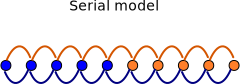
\includegraphics[width=0.24\linewidth]{serial.svg}}
      &
      \item\label{fig:binary_ChR2}
      \hspace{0.05\linewidth}\aligntop{\includegraphics[width=0.12\linewidth]{binary.svg}}
      &
      \item\label{fig:multistate_ChR2}
      \aligntop{\includegraphics[width=0.24\linewidth]{multistate.svg}}
      \\[1.3cm]
      \aligntop{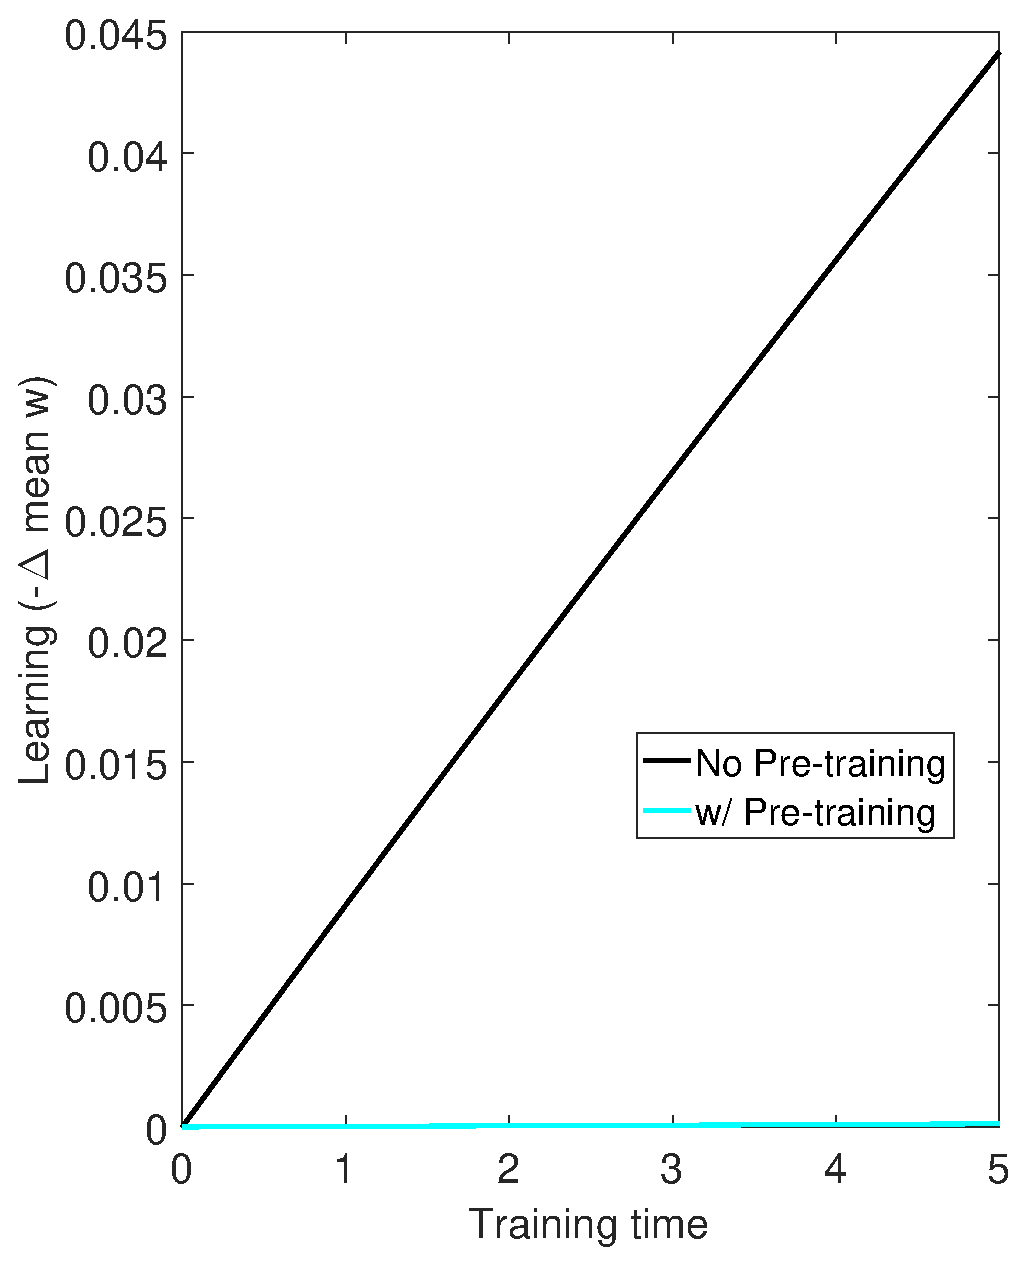
\includegraphics[width=0.29\linewidth]{serial_fit_ChR2_learnS.eps}}
      &
      \aligntop{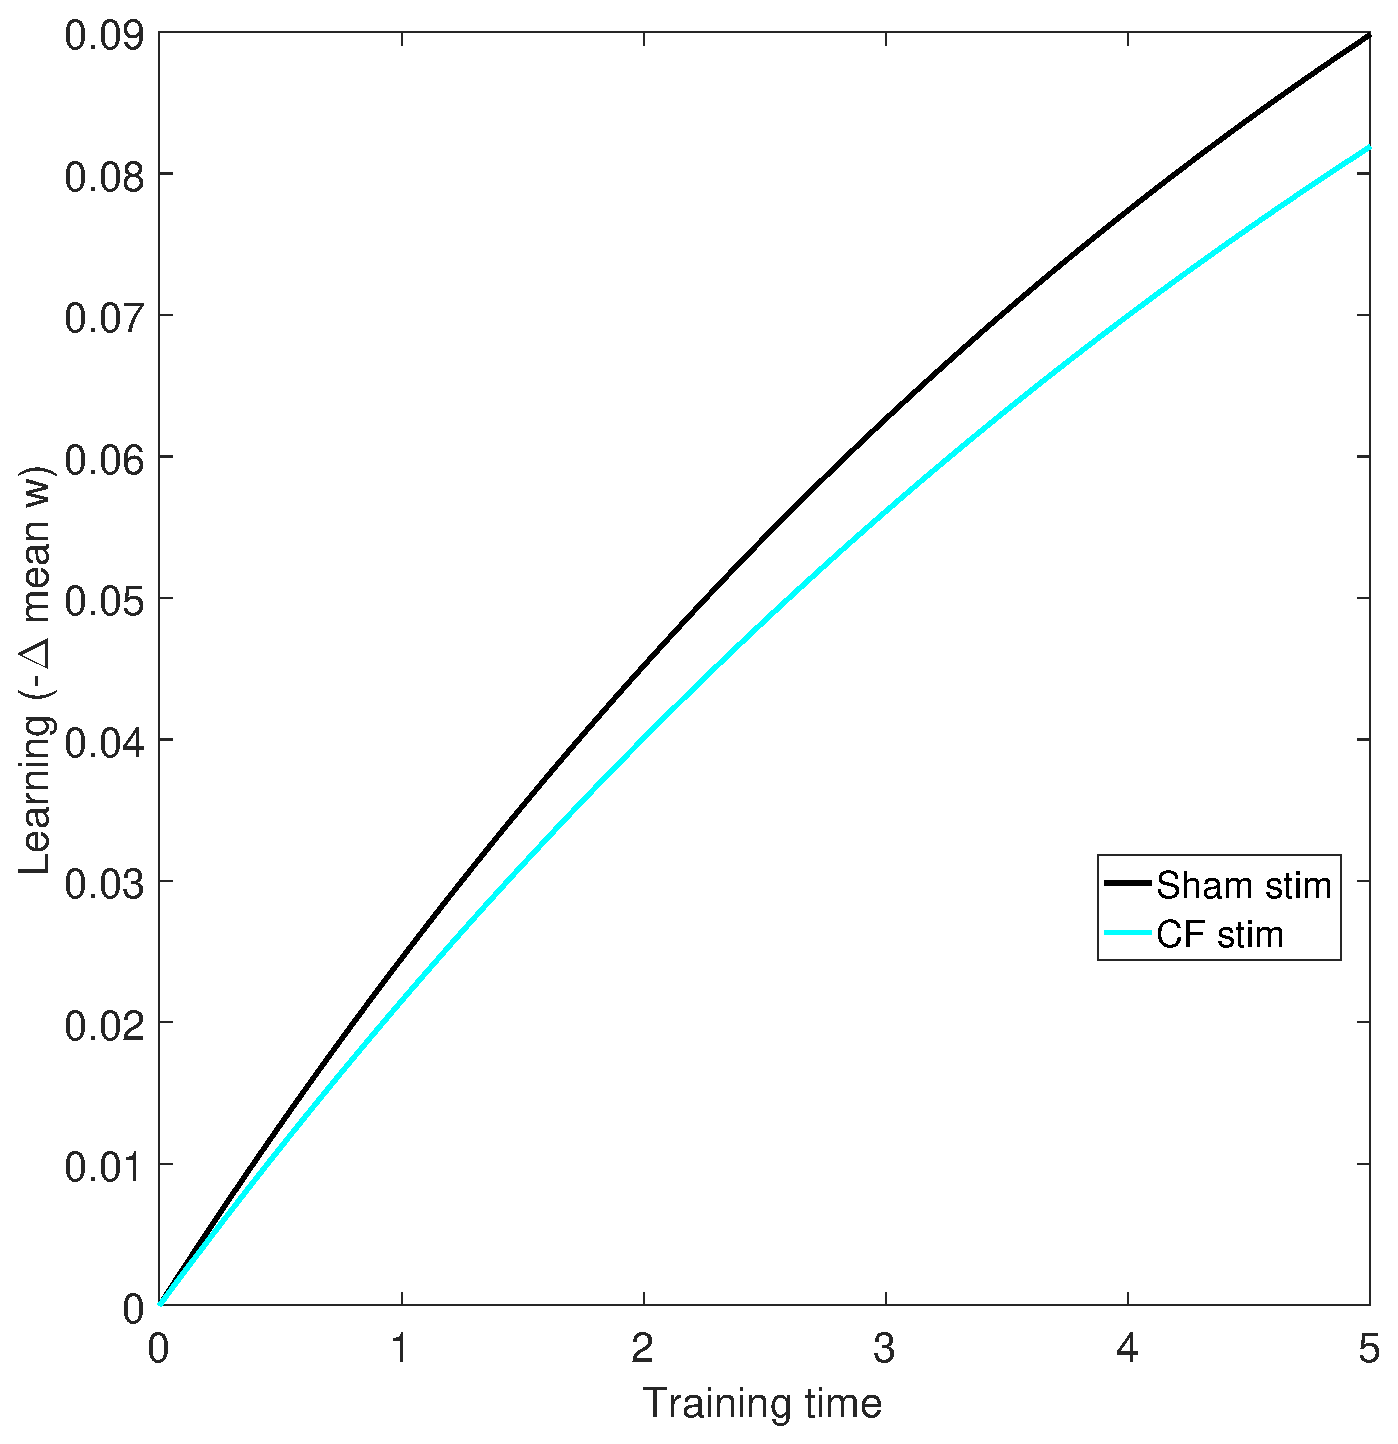
\includegraphics[width=0.29\linewidth]{binary_ChR2_learnS.eps}}
      &
      \aligntop{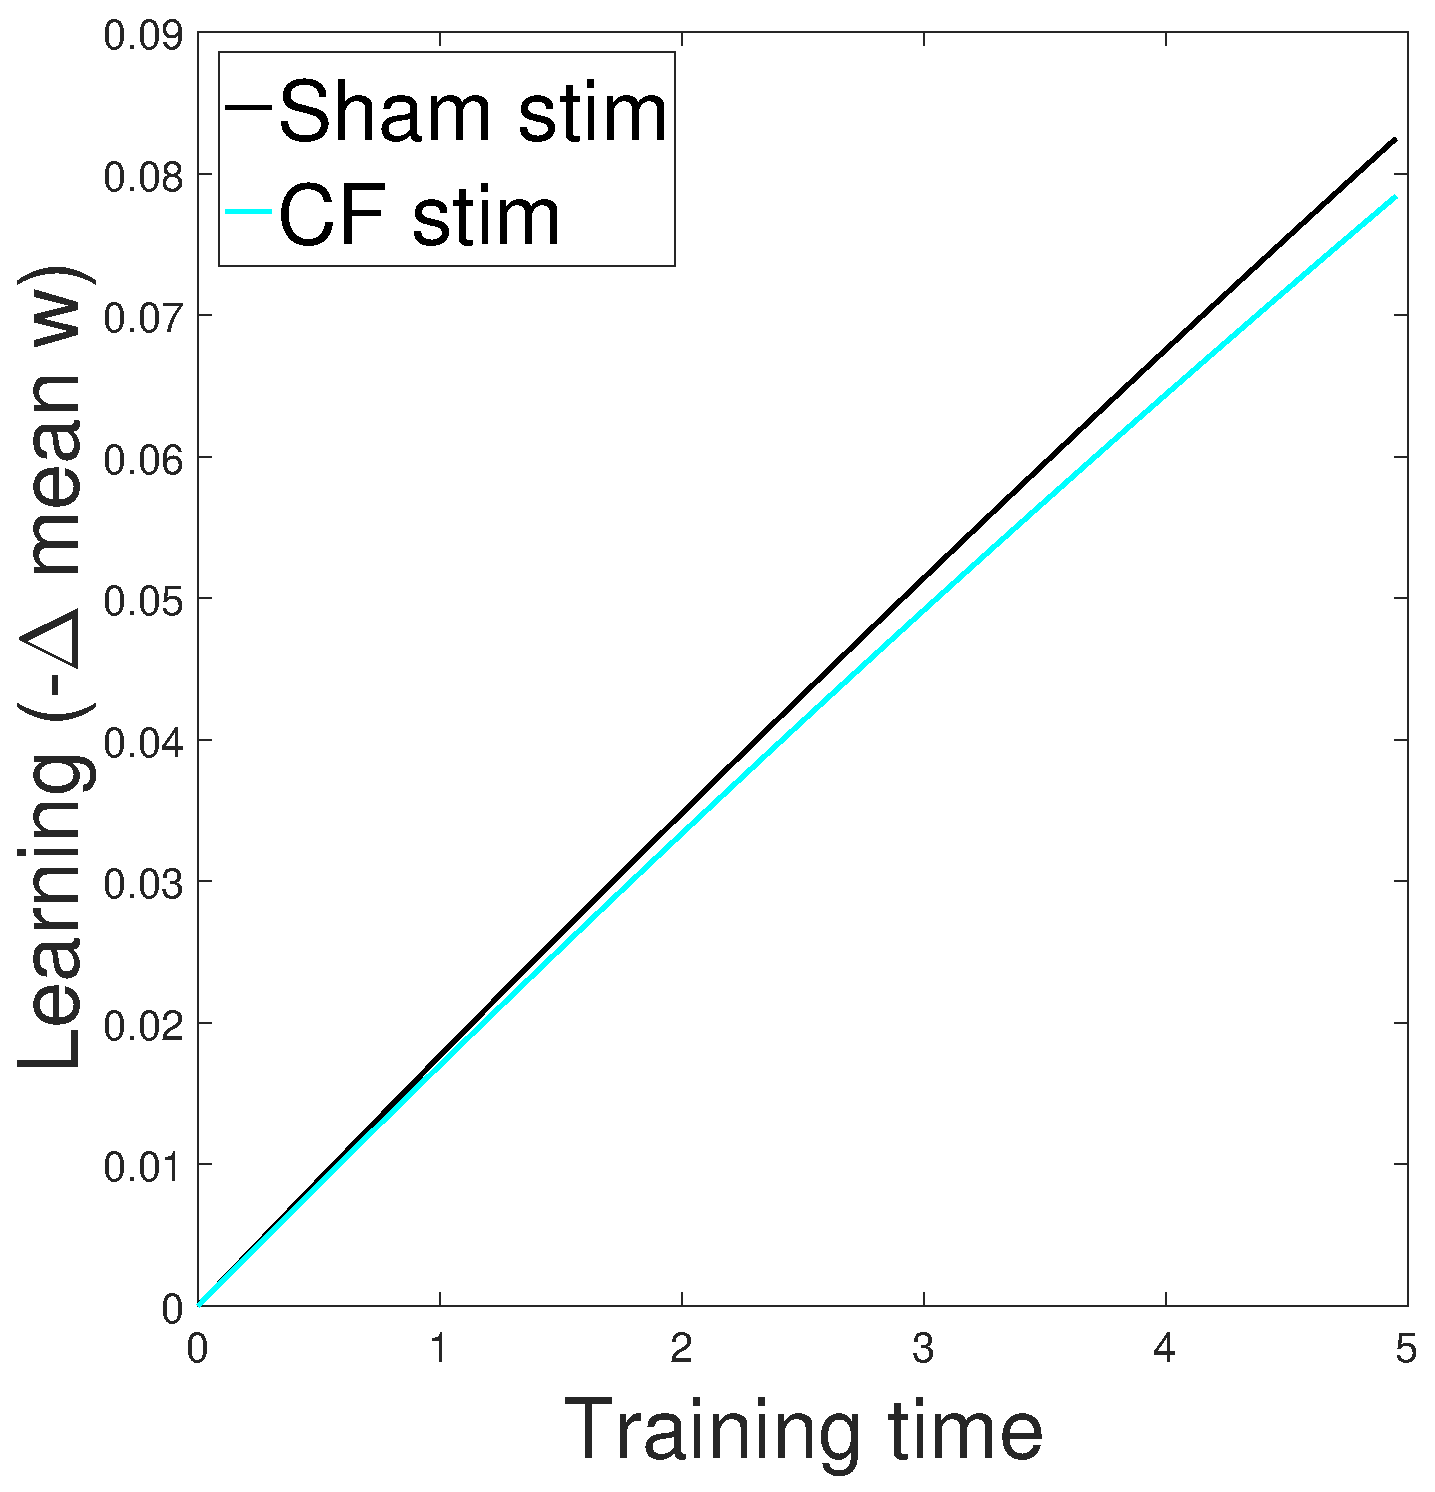
\includegraphics[width=0.29\linewidth]{multistate_lin_ChR2_learnS.eps}}
      \\[4.5cm]
      \item\label{fig:pooled_ChR2}
      \aligntop{\includegraphics[width=0.29\linewidth]{pooled_deponly.svg}}
      &
      \item\label{fig:cascade_ChR2}
      \aligntop{\includegraphics[width=0.24\linewidth]{cascade.svg}}
      &
      \item\label{fig:nonuni_ChR2}
      \aligntop{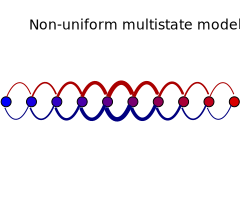
\includegraphics[width=0.24\linewidth]{multistate_nonuni.svg}}
      \\[1.8cm]
      \aligntop{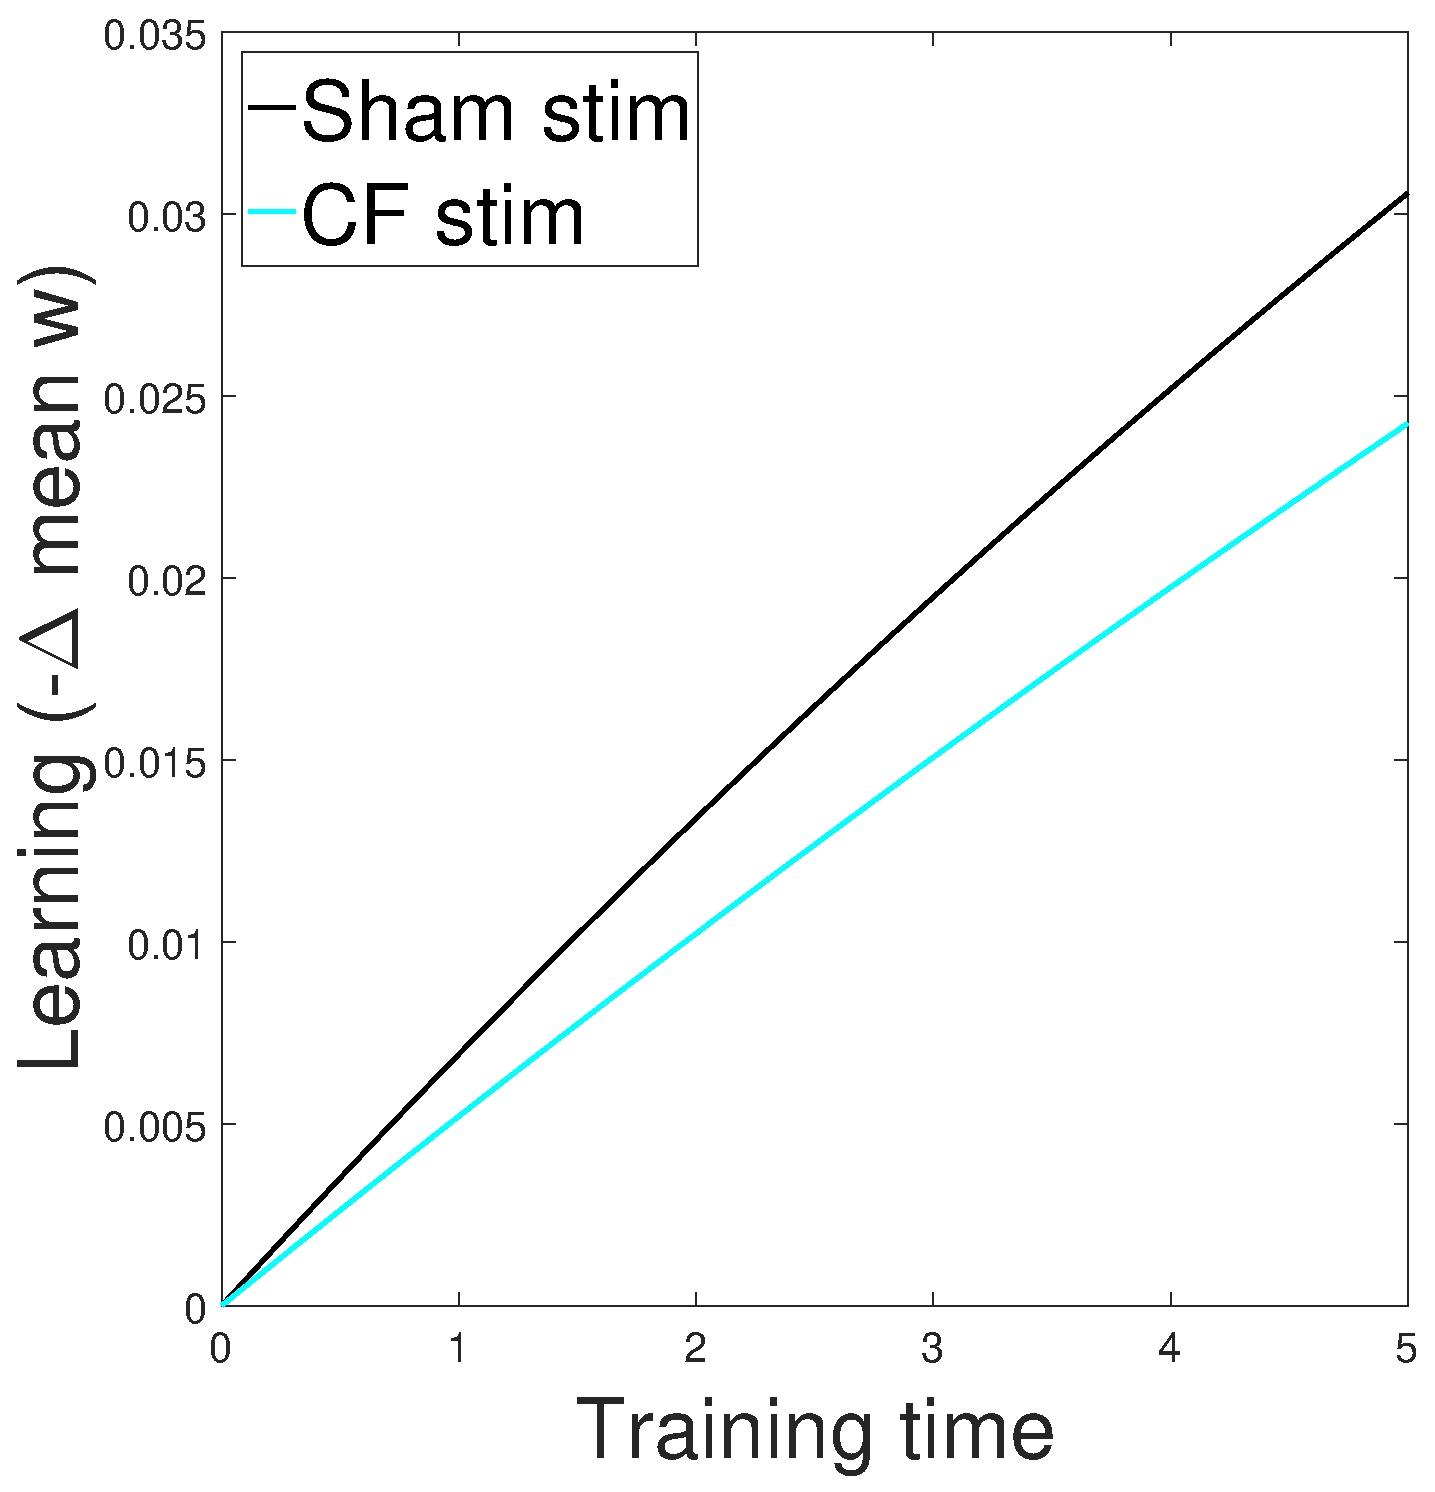
\includegraphics[width=0.29\linewidth]{pooled_deponly_ChR2_learnS.eps}}
      &
      \aligntop{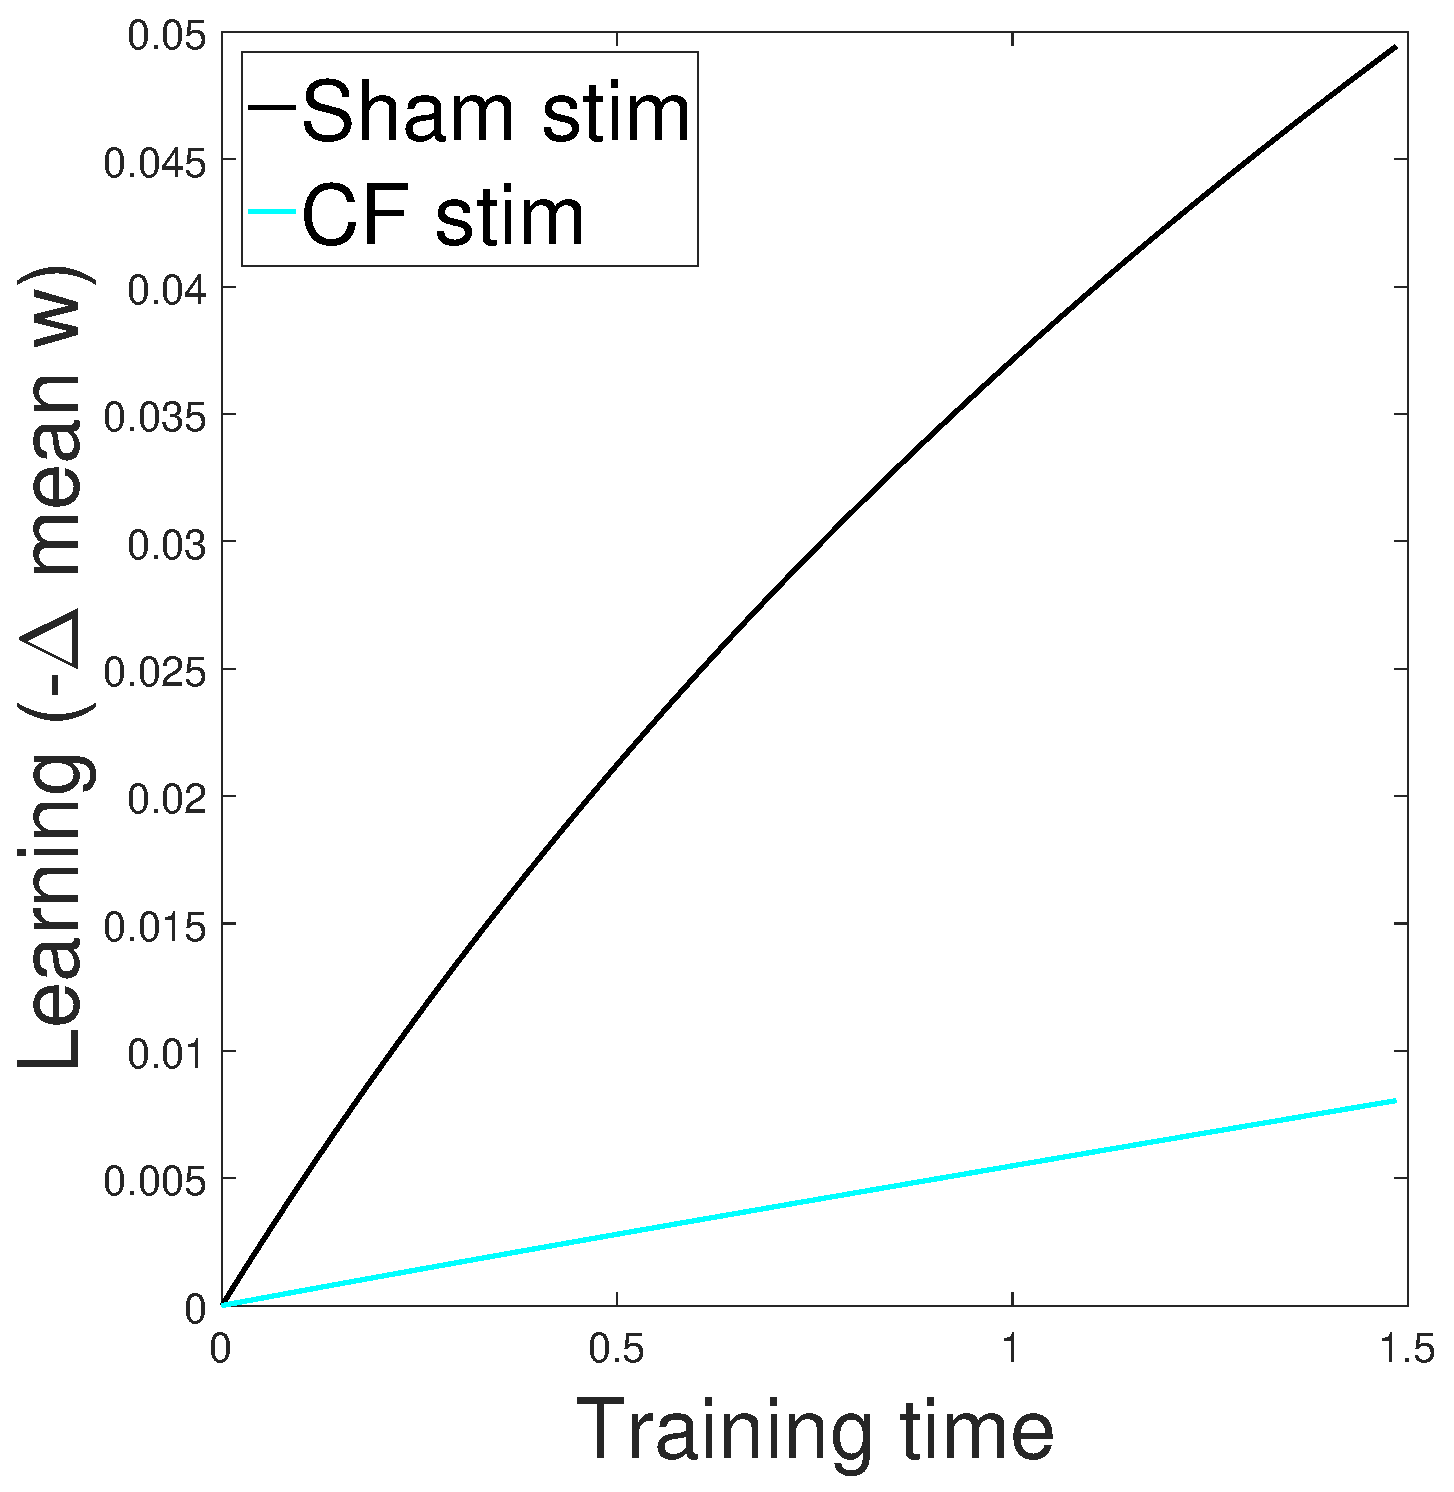
\includegraphics[width=0.29\linewidth]{cascade_fit_ChR2_learnS.eps}}
      &
      \aligntop{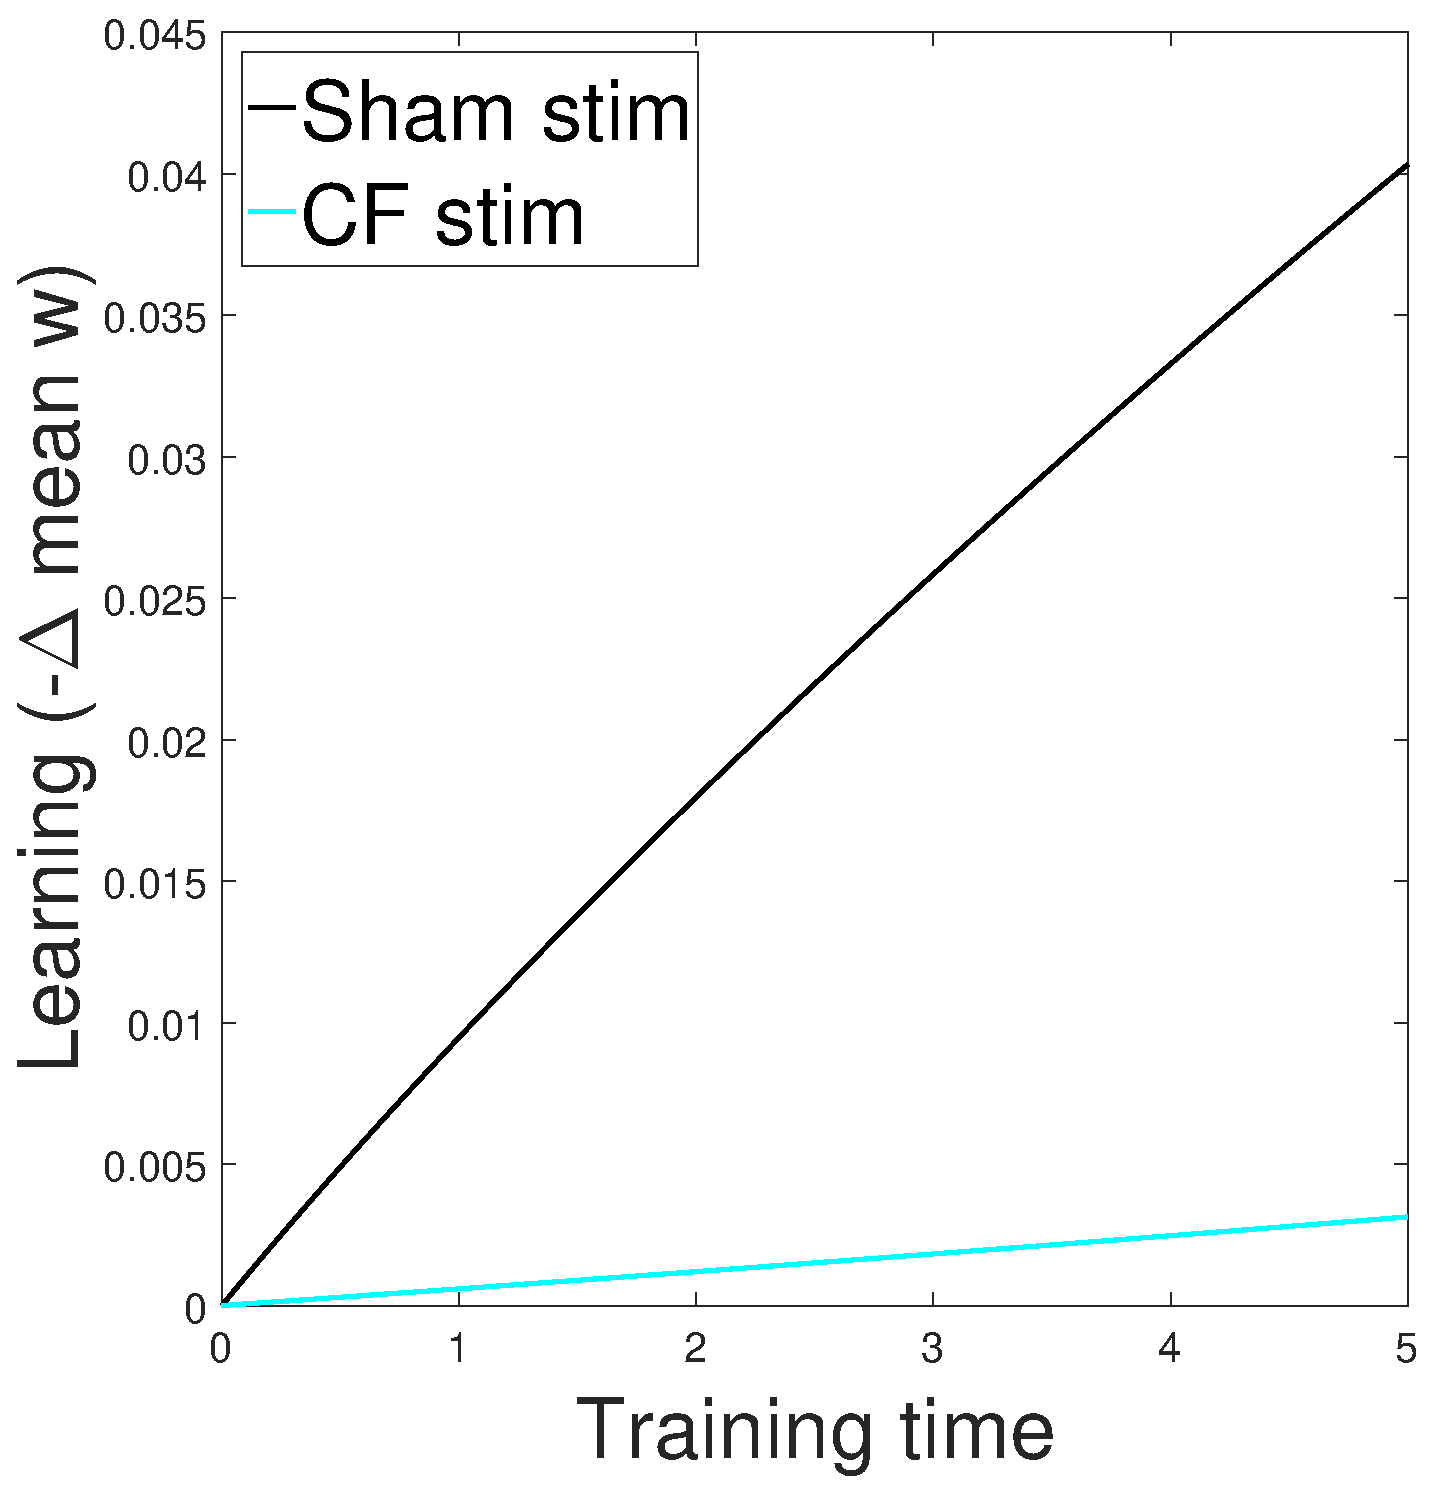
\includegraphics[width=0.29\linewidth]{nonuni_fit_ChR2_learnS.eps}}
  \end{tabular}

  \vspace{0.5cm}
  \item\label{tab:params_ChR2}\aligntop{
  \begin{tabular}{|l|c|c|c|c|c|c|c|}
    \cline{1-8}
    % after \\: \hline or \cline{col1-col2} \cline{col3-col4} ...
    Model & \#  & \multicolumn{2}{c|}{Plasticity param.} & \multicolumn{3}{c|}{$f\dep$} & $r\tpre$ \\
    \cline{3-7}
    & states & pot & dep & base & inc & CF Stim & {} \\

    \cline{1-8}
    Serial       & 10 & $0.12$  & $0.14$        & 0.5   & 0.89 & 0.9879 & 100 \\
    Two-state    & 2  & $0.1$   & $0.4$         & 0.5   & 0.7  & 0.91   & 5   \\
    Multistate   & 10 & $0.3$   & $0.3$         & 0.5   & 0.8  & 0.96   & 5   \\
    Pooled res.\ & 7  & $0.08$  & $[0.006,0.6]$ & 0.5   & 0.9  & 0.99   & 20  \\
    Cascade      & 14 & $0.386$ & $0.398$       & 0.522 & 0.63 & 0.99   & 200  \\
    Non-uni.\    & 12 & $0.4$   & $0.4$         & 0.5   & 0.7  & 0.99   & 500  \\
    \cline{1-8}
  \end{tabular}}
  \end{myenuma}
  \caption[Simulation results for various models]{(\ref{fig:serial_ChR2}-\ref{fig:nonuni_ChR2}) Simulation results for various models, showing decrease in mean synaptic weight over time during gain increase training from the normal state (black) and after non-specific CF stimulation (cyan) for wild-type models.
  (\ref{tab:params}) Parameters used for simulations.
  For the serial, two state and multistate models, the plasticity parameter listed is the transition probability between adjacent states.
  For the pooled resource model, the plasticity parameters are the minimum and maximum transition probability for the constituent two-state synapses.
  For the cascade and non-uniform multistate models, the plasticity parameter is the ratio of adjacent transition probabilities.}\label{fig:sim_ChR2}
\end{figure}


Here, we model the effects of non-specific climbing fibre stimulation, as in \chrfig.
It is necessary to also model the ``other'' population of synapses that compensate for the change in baseline synaptic weight of the synapses considered up to now, either due to enhanced plasticity or non-specific CF stimulation.

To be concrete, we model these other synapses as described in \compfig.
We set the relative rate of depression events for these synapses during training to $f\dep = f\dep\norm$, \ie the baseline value, so that they are unaffected by training.
Here we set the rate of plasticity events causing forgetting of the CF stimulation in these synapses is the same as the rate of plasticity events in the original synapses during training, although similar results could be acheived with other choices.
For both sets of synapses during non-specific CF stimulation, we set $f\dep > f\dep\norm$ to model the increased rate of depression.
The values of all parameters used can be seen in \autoref{fig:sim_ChR2}\ref{tab:params_ChR2}.

In \autoref{fig:sim_ChR2}\ref{fig:serial_ChR2}--\ref{fig:nonuni_ChR2} we see examples of simulations of all of the models we have considered.
We see that every single one of them is capable of reproducing the experimental results of \chrfig, for suitable parameter choices.
This is because this intervention has the effect of depleting the population of synapses available for depression \emph{without} the competing effect of enhanced plasticity.
Therefore the depletion effect is stronger (than 0) and learning is impaired.
This means that these experiments cannot rule out any of the models.
However these experiments do agree with the idea of impaired learning due to depletion of the population of labile synapses.


%%%%%%%%%%%%%%%%%%%%%%%%%%%%%%%%%%%%%%%%%%%%%%%%%%%%%%%%%%%%%%%%%%%%%%%%%%

\section{Balanced potentiation and depression}\label{sec:bal}


As the baseline oculomotor performance was normal in the \KO\ mice (see \basefig), one might ask if it is possible that potentiation is also enhanced by the knockout, in such a way that the baseline mean synaptic weight is unchanged.

Intuitively, this seems impossible.
The impaired learning observed in some of the models considered depended on the competition between the enhanced intrinsic plasticity rate and the depletion of the population of synapses available for depression.
If the second effect is removed, the first must dominate and learning will be enhanced.

However, enhancing potentiation will increase the number of synapses making transitions in the ``wrong'' direction, impairing learning.
Furthermore, the distribution of synapses across labile and stubborn states may be altered, also affecting the learning rate.

For the \hyperref[sec:multistate]{serial}, \hyperref[sec:binary]{two-state} and \hyperref[sec:multistate_lin]{multistate} models, the validity of the intuition can be seen analytically.
From \eqref{eq:mutltieq}, we can see that the baseline mean synaptic weight depends monotonically on the quantity
%
\begin{equation*}
  \alpha=\frac{f\pot q\pot}{f\dep q\dep}.
\end{equation*}
%
Maintaining the same baseline would then require increasing $q\pot$ in proportion to $q\dep$.
As one can see from \eqref{eq:multiflux}, \eqref{eq:binaryflux} and \eqref{eq:multiLinFlux}, this will always lead to an enhanced initial learning rate.

For the other models, a numerical analysis is required, as shown in \autoref{fig:bal}.
\hypertarget{par:bal_scan}{To} see if learning is impaired with enhanced plasticity each relevant parameter was scanned over 10 values from 0.05 to 0.95, rejecting values that do not respect the inequalities:
$0 \leq f\dep\norm < f\dep\inc \leq 1$, for the pooled resource model $0 \leq q\dep_\text{min,WT} < q\dep_\text{min,\KO}, q\dep_\text{max,WT} < q\dep_\text{max,\KO}$ and $0 \leq q\pot\wt$, for the cascade model $0 \leq x\dep\wt < x\dep\ko \leq \frac{1}{2}$ and $0 \leq x\pot\wt \leq \frac{1}{2}$, and for the nonuniform multistate model $0 \leq x\dep\wt < x\dep\ko \leq 1$ and $0 \leq x\pot\wt \leq 1$.
In each case, the \KO\ potentiation parameter, $q\pot\ko$ for the pooled resource model and $x\pot\ko$ for the others, was adjusted to match the baseline mean synaptic weight. $\pr(0)\w$, with wild-type.

We see that, for most parameter values, such models do not reproduce the observed learning impairment with enhanced plasticity.
In some cases a very small learning impairment was seen ($\CO(10^{-5})$), but these occurred at extreme parameter values where the tolerances used in fitting the potentiation parameter could have a noticeable impact.

%We see that, for all parameter values, such models do not reproduce the observed learning impairment with enhanced plasticity.
%The normal baseline oculomotor performance must have some other explanation, such as those outlined in \compfig.




\begin{figure}
  \centering
  \begin{myenuma}
    \item\aligntop{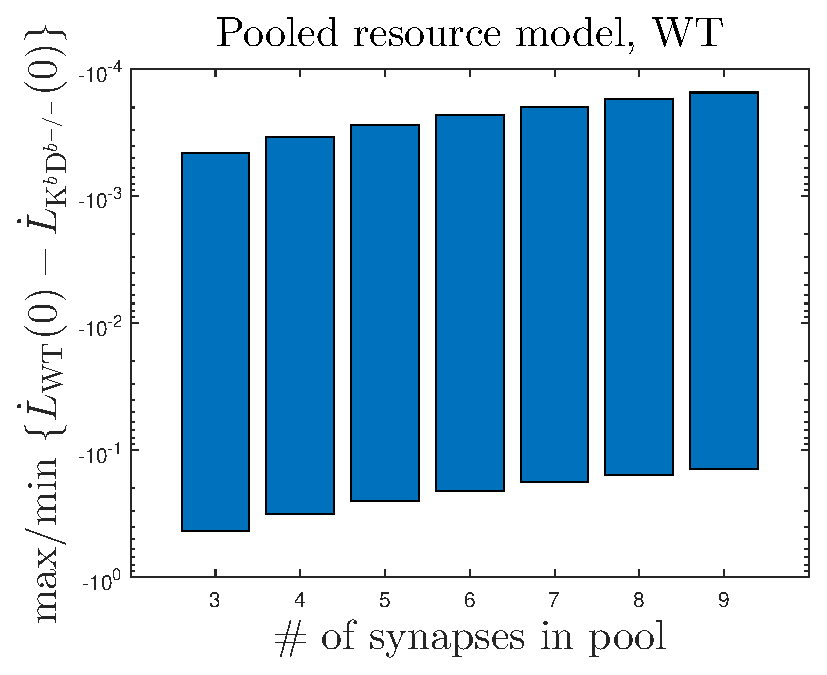
\includegraphics[width=0.29\linewidth]{pooled_scan.eps}}\label{fig:pooled_bal}
    \item\aligntop{\includegraphics[width=0.29\linewidth]{cascade_scan.eps}}\label{fig:cascade_bal}
    \item\aligntop{\includegraphics[width=0.29\linewidth]{nonuni_scan.eps}}\label{fig:nonuni_bal}
  \end{myenuma}
  \caption{Difference in initial learning rate in wild-type and \KO\ models, without gain-decrease pre-training.
  Learning, $L(t)$ is defined in \eqref{eq:learning}.
  Here, we show the maximum and minimum values of this quantity when scanning all 7/5 relevant parameters (see \protect\hyperlink{par:bal_scan}{text}).
  We see that this quantity is usually negative, whereas it was positive in the experiments.
  The exceptions are very small, $\CO(10^{-5})$, and tend to occur at extreme parameter values where the accuracy of fitting the potentiation parameter could become an issue.
  }\label{fig:bal}
\end{figure}





%%%%%%%%%%%%%%%%%%%%%%%%%%%%%%%%%%%%%%%%%%%%%%%%%%%%%%%%%%%%%%%%%%%%%%%%%%

\bibliographystyle{utcaps_sl}
\bibliography{neuro,markov}

\end{document}
